\chapter{Ejemplos de uso extensos} \label{chp:anexo_docs_examples}

En este anexo se encuentran ejemplos elaborados para demostrar el uso de las propuestas en un contexto más cercano a la realidad. Se muestran en forma de imágenes, pues es lo que una persona usuaria final vería.

En las propuestas aceptadas se podrá descargar el código fuente de la misma página. En el caso de las no aceptadas, habría que acceder a la \gls{rama} de trabajo de la propuesta mediante la \textit{\gls{pull request}} correspondiente o la página de la documentación que se aloja temporalmente en la web, si es que existe.

%%%%%%%%%%%%%%%%%%%%%%%%%%%%%%%%%%%%%%%%%%%%%%%%%%%%%%%%%%%%%%%%%%%%%%%%%%%%%%%%
\begin{myparindent}{0pt}

\newpage\section{Modelo de ajuste espectral} \label{sct:doc_ej_modelo_nuria}

Propuesta en \pr{1658}, no aceptada.

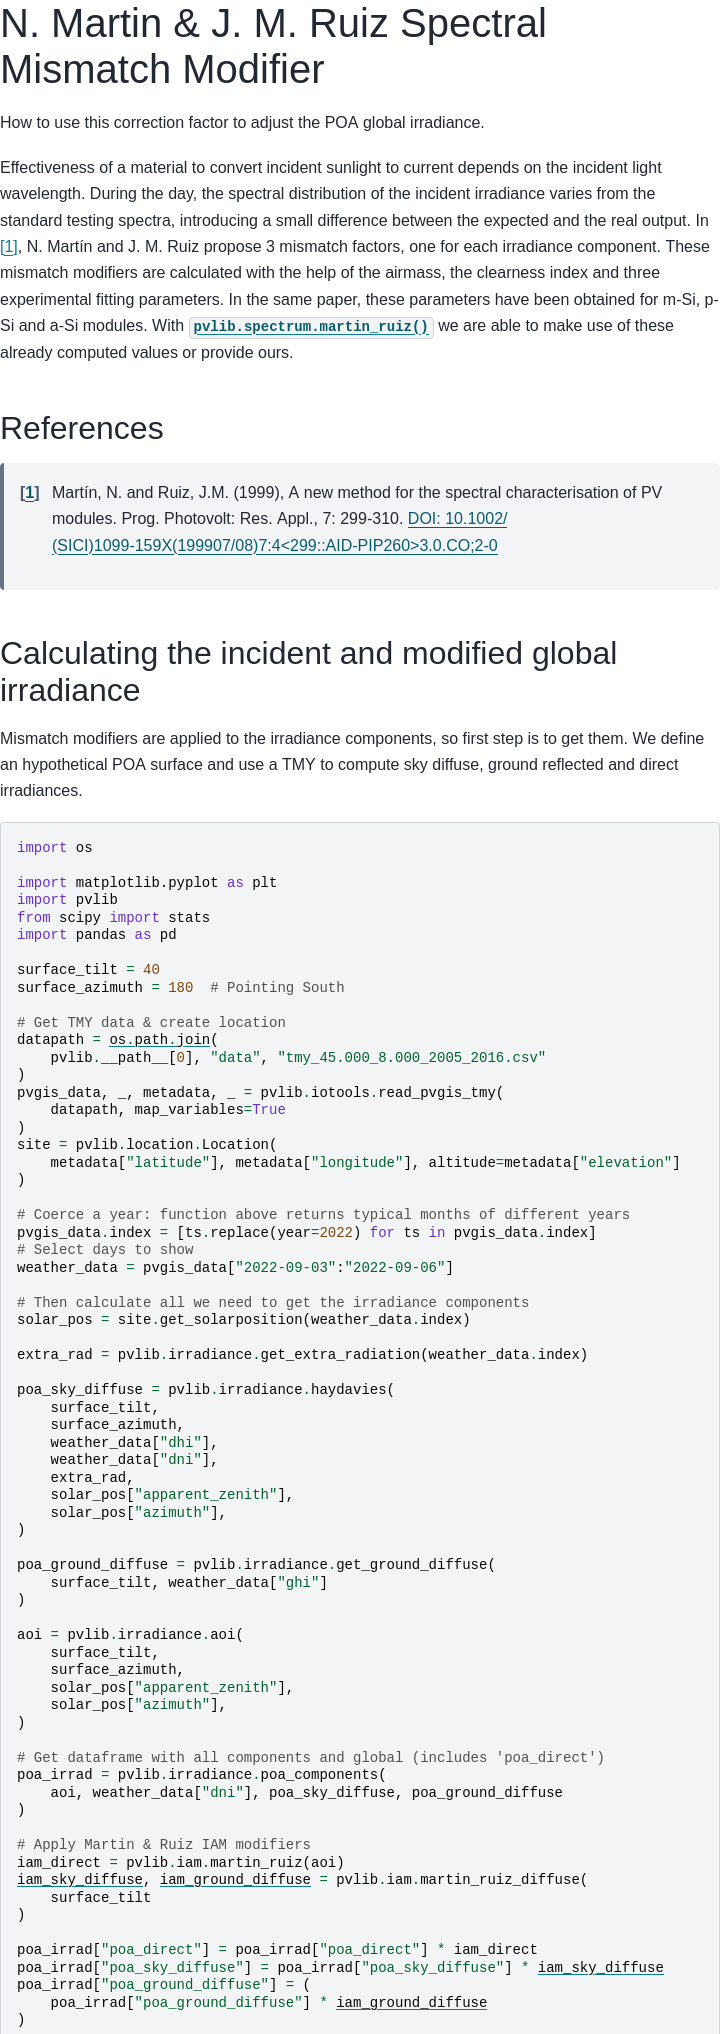
\includegraphics[width=\linewidth,height=0.9\textheight,keepaspectratio]{images/docs_examples_cut/mr_0.png}

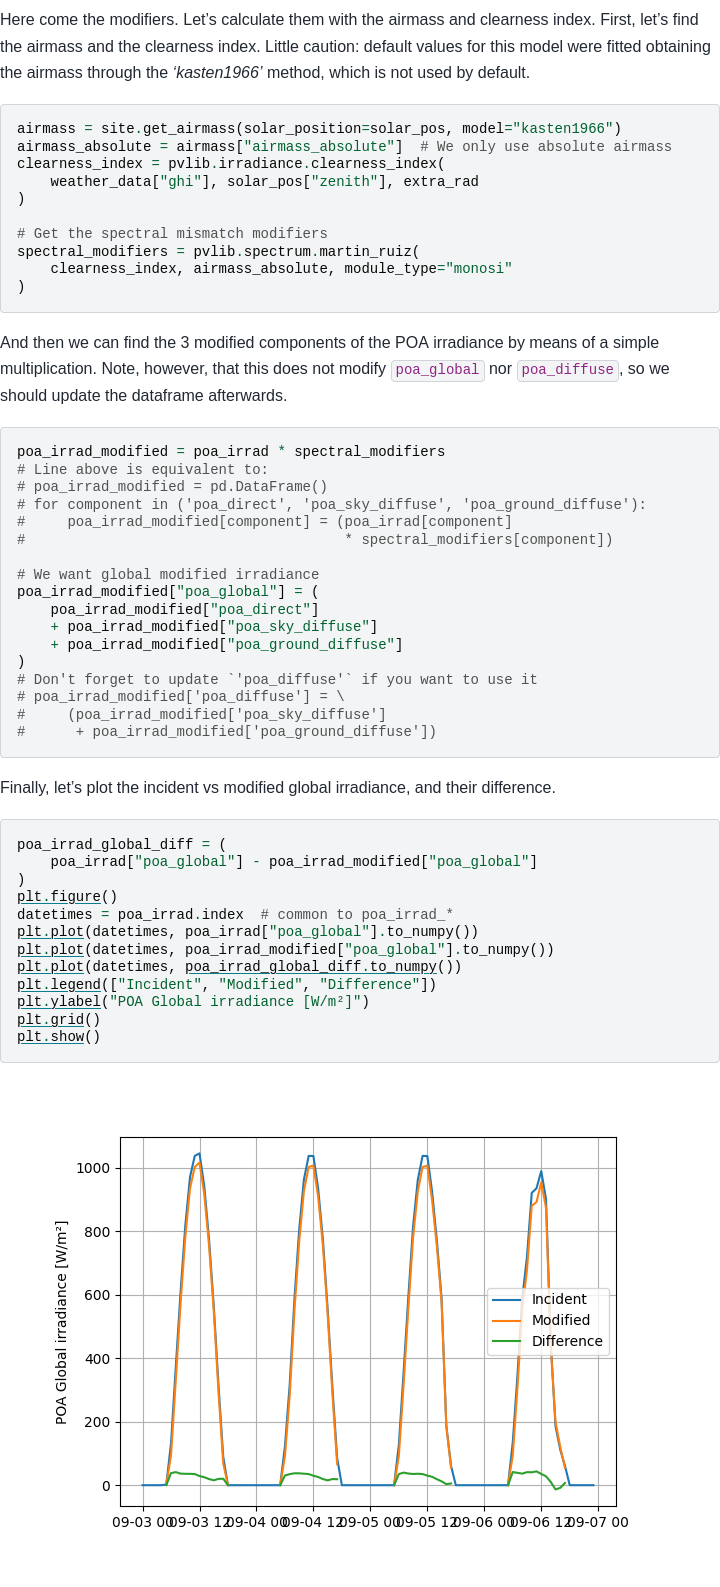
\includegraphics[width=\linewidth,height=0.9\textheight,keepaspectratio]{images/docs_examples_cut/mr_1.png}

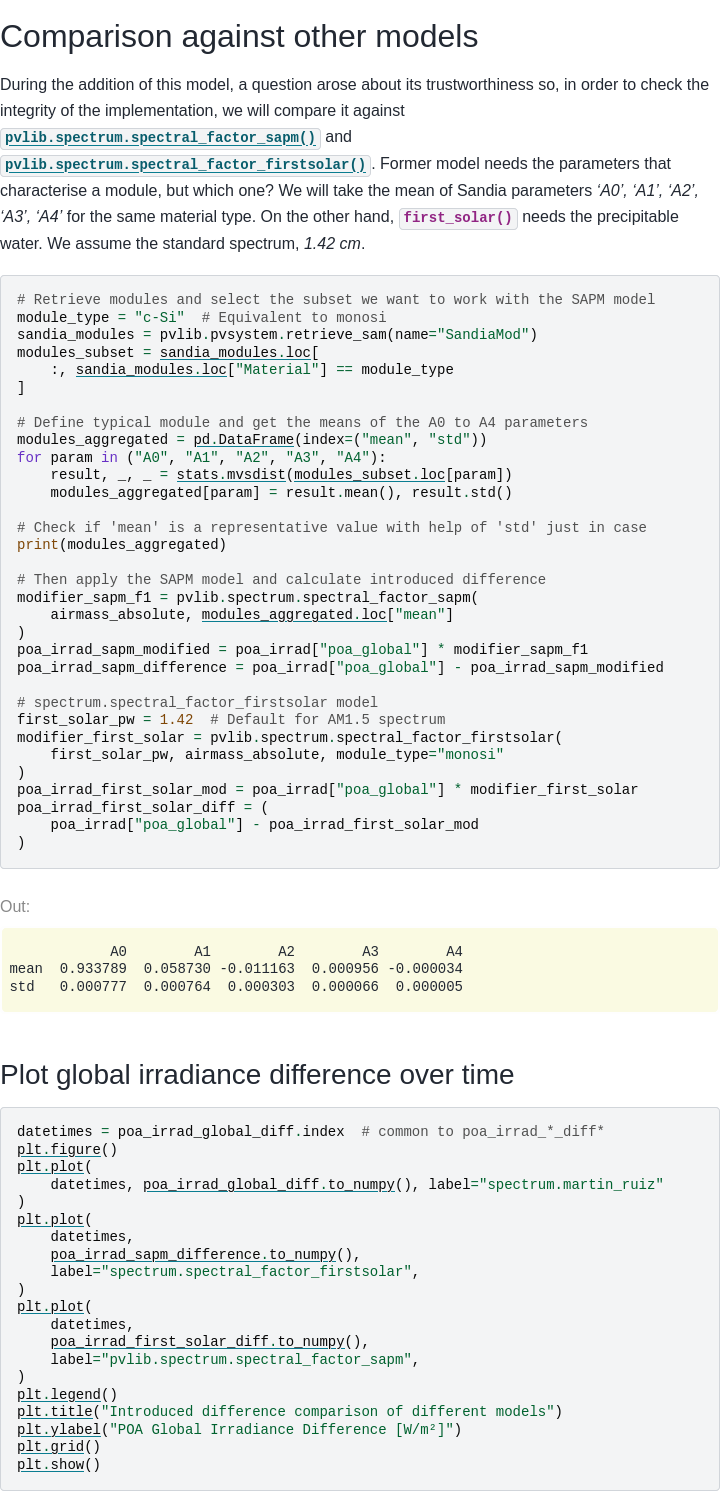
\includegraphics[width=\linewidth,height=0.9\textheight,keepaspectratio]{images/docs_examples_cut/mr_2.png}

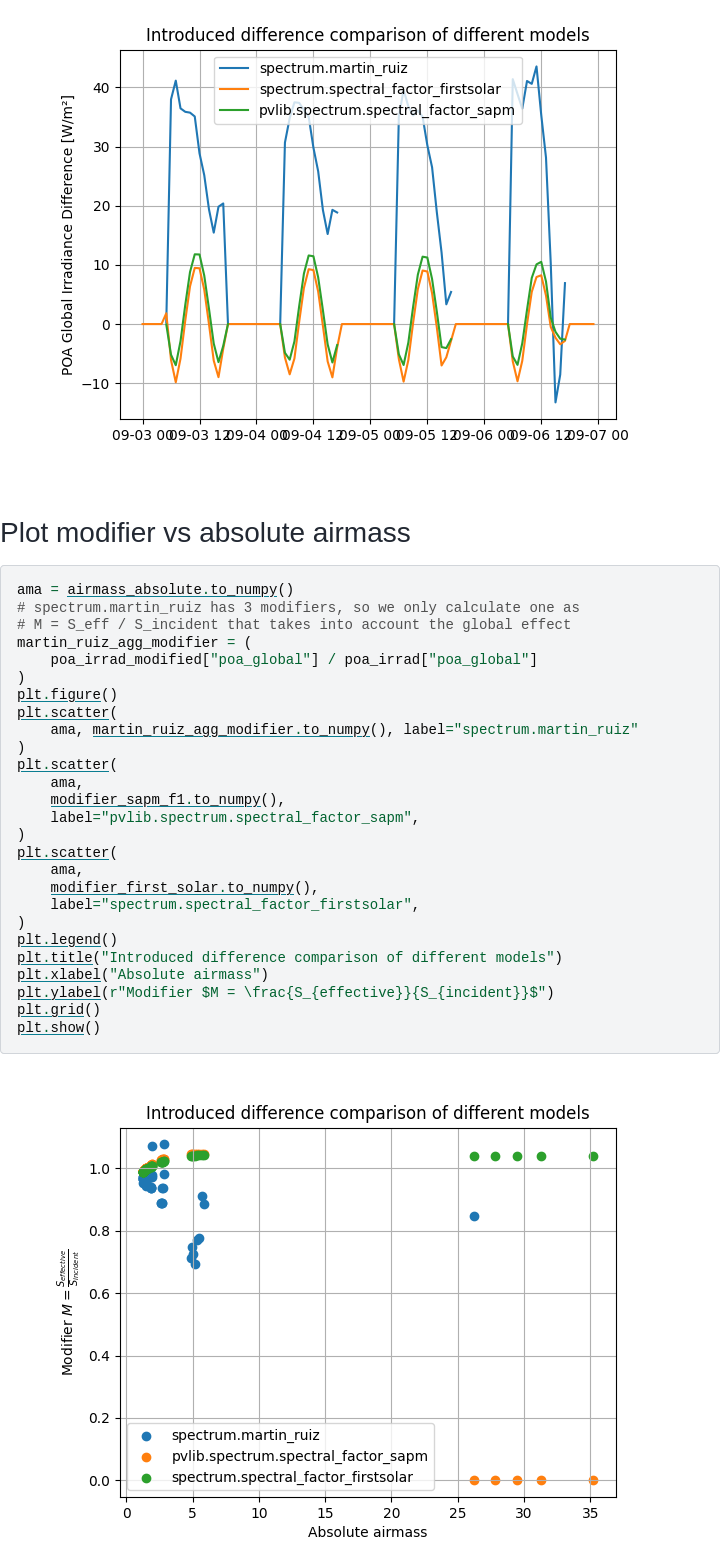
\includegraphics[width=\linewidth,height=0.9\textheight,keepaspectratio]{images/docs_examples_cut/mr_3.png}

\newpage\section{Fracción de sombra unidimensional} \label{sct:doc_ej_fraccion_sombra}

\pr{1962}, acceso a ejemplo en \href{https://pvlib-python.readthedocs.io/en/stable/gallery/shading/plot_shaded_fraction1d_ns_hsat_example.html}{este link}.

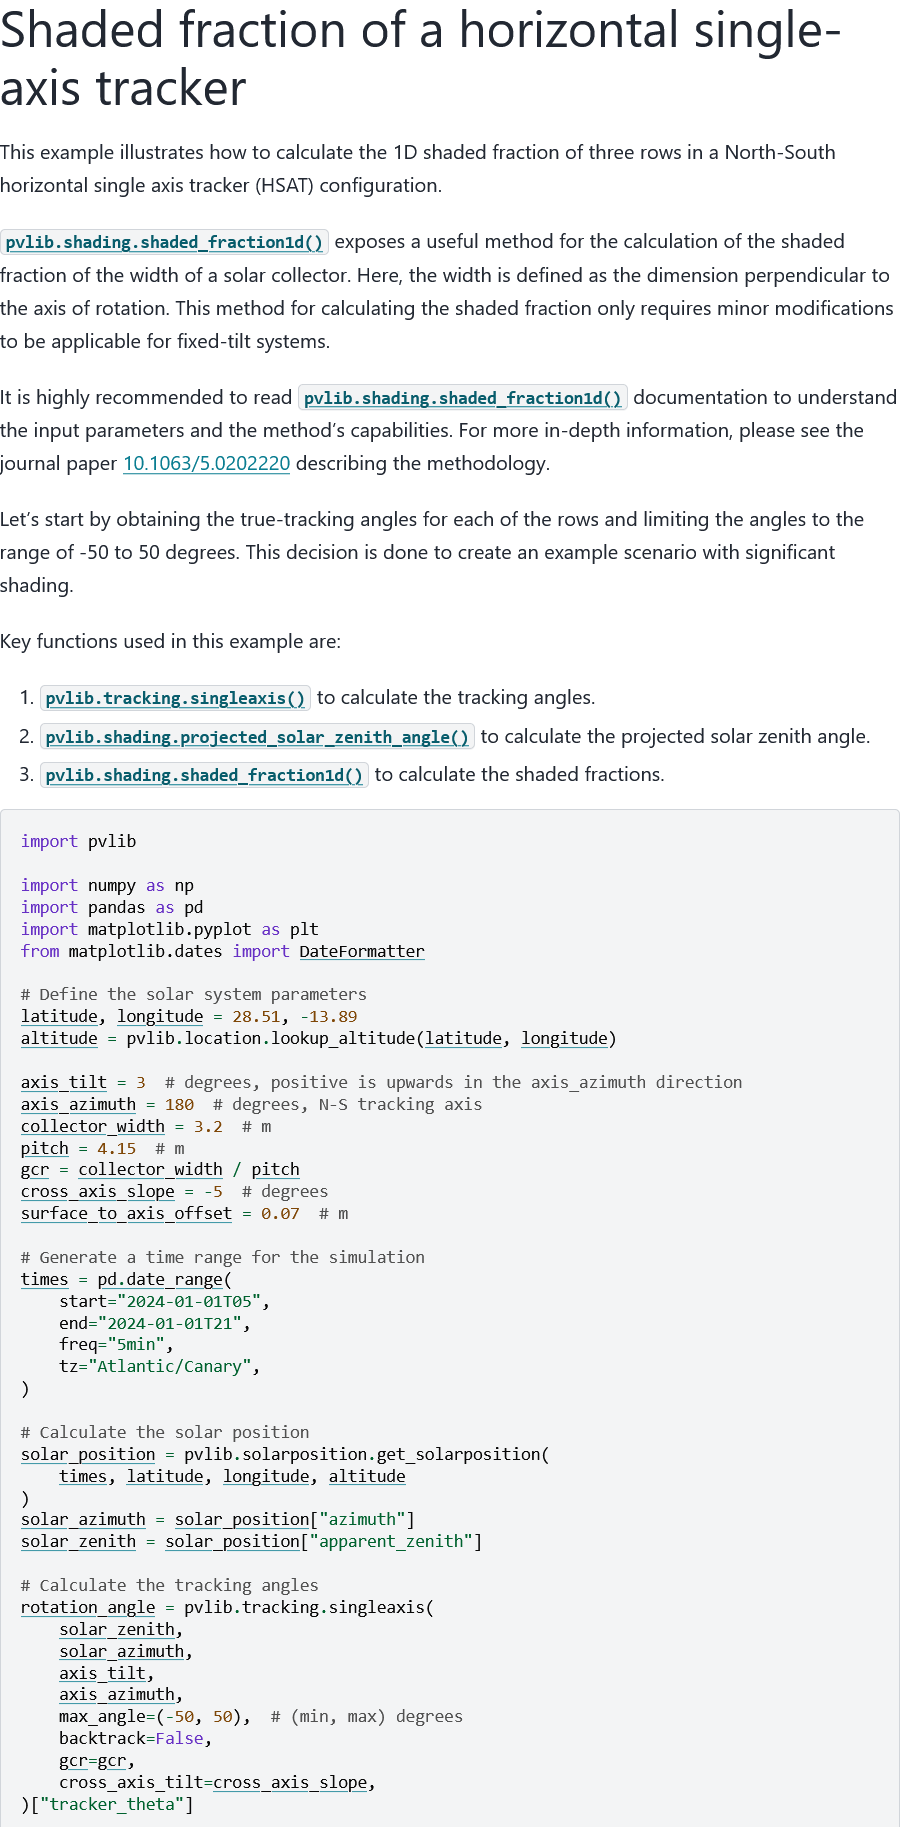
\includegraphics[width=\linewidth,height=0.9\textheight,keepaspectratio]{images/docs_examples_cut/shaded_fraction_0.png}

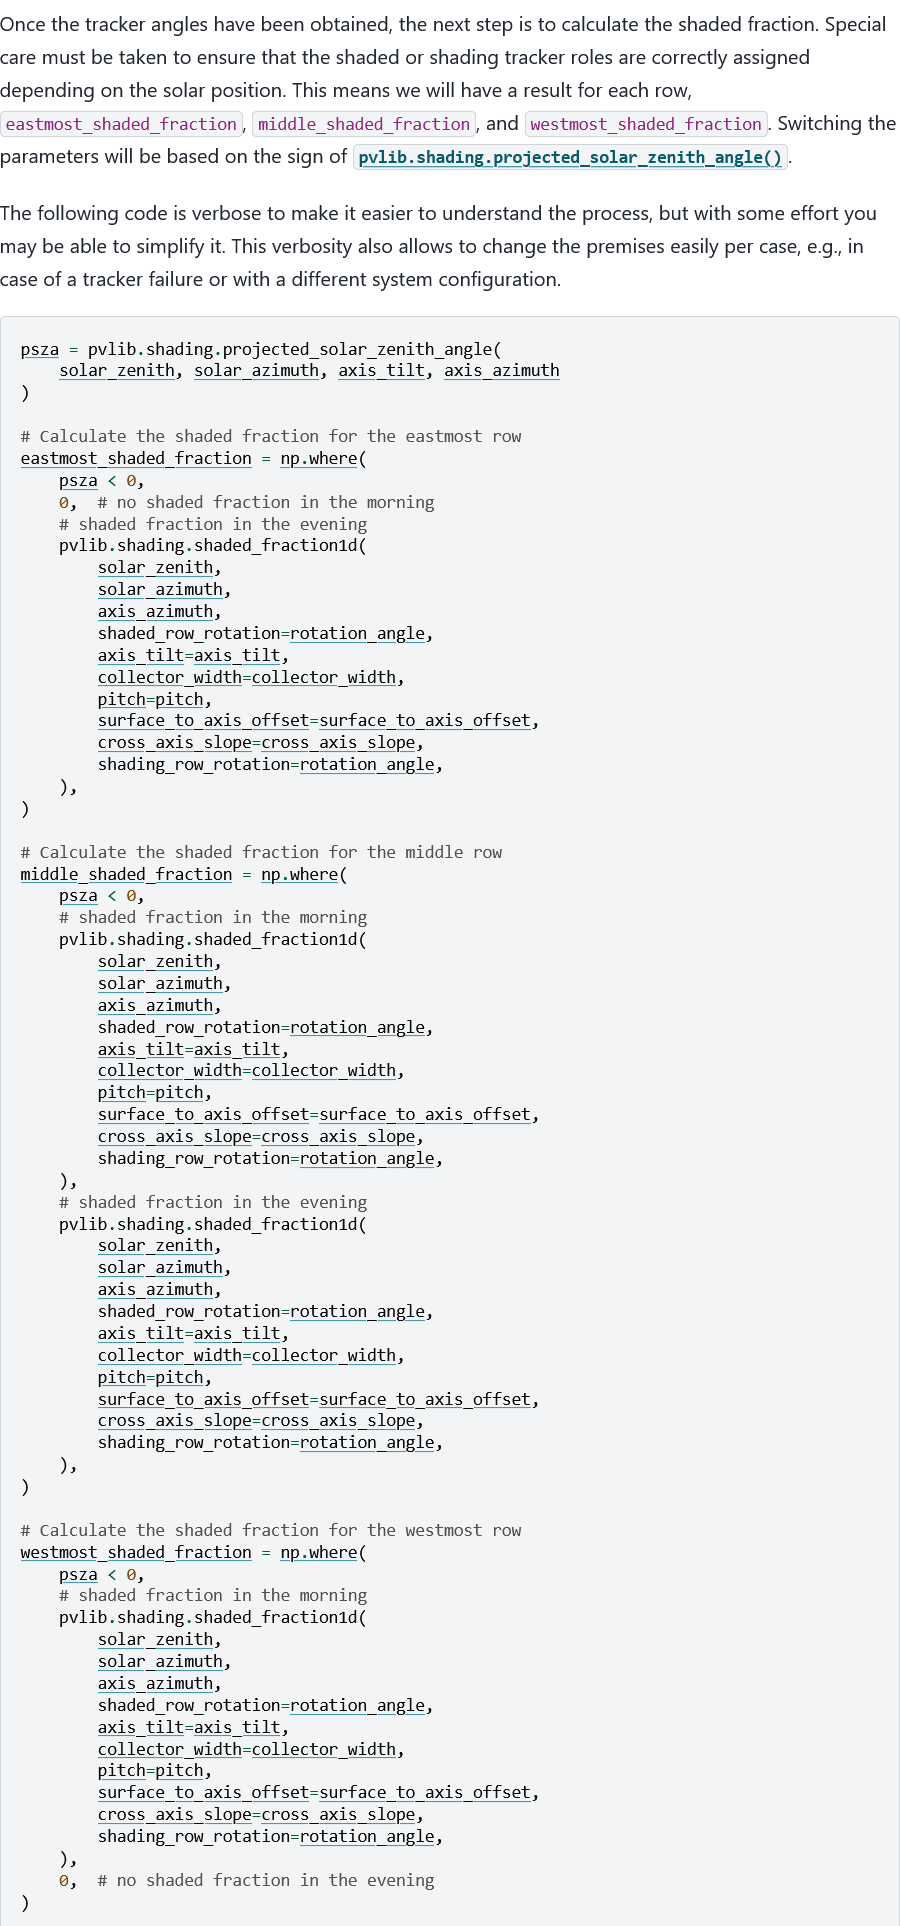
\includegraphics[width=\linewidth,height=0.9\textheight,keepaspectratio]{images/docs_examples_cut/shaded_fraction_1.png}

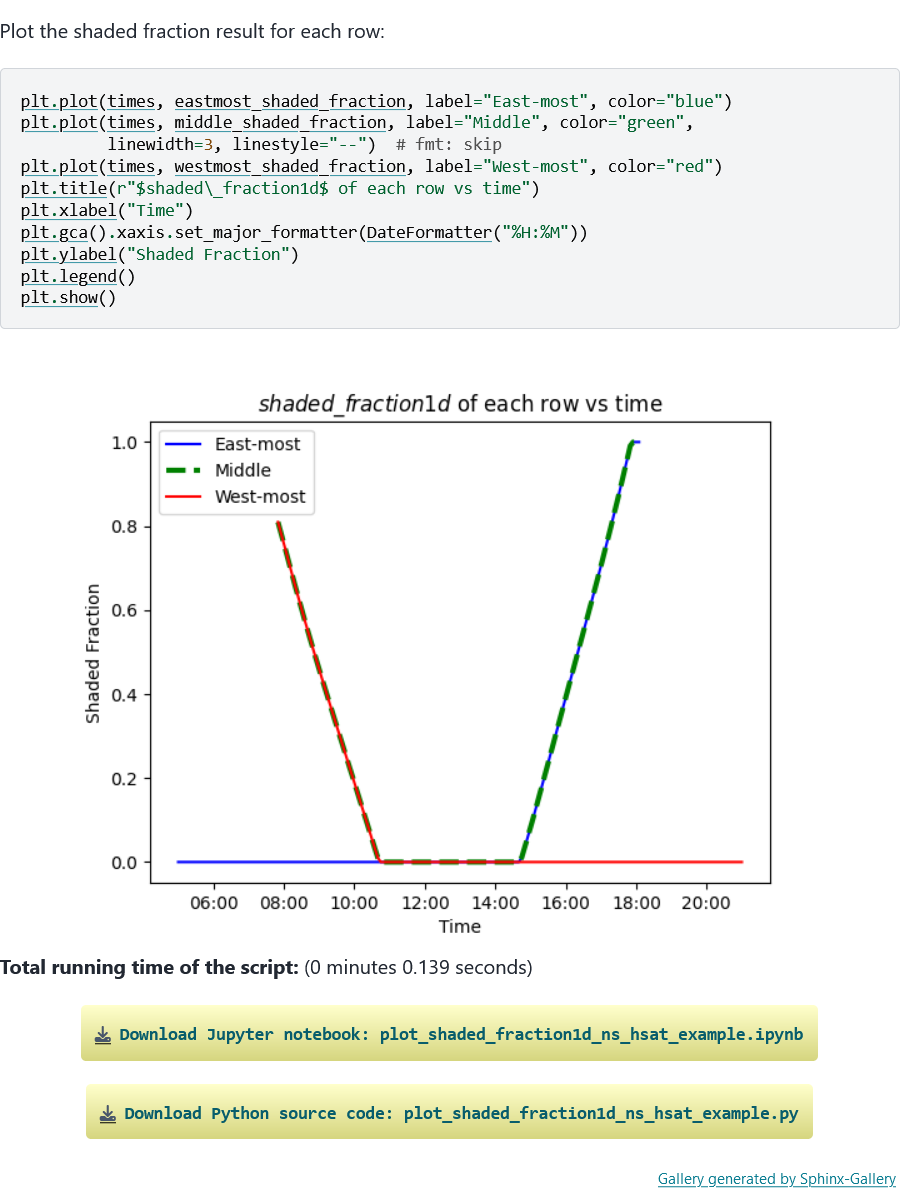
\includegraphics[width=\linewidth,height=0.9\textheight,keepaspectratio]{images/docs_examples_cut/shaded_fraction_2.png}

\newpage\section{Pérdidas por sombras en módulos con diodos de bypass} \label{sct:doc_ej_perdidas_sombra}

\pr{2070}, acceso a ejemplo en \href{https://pvlib-python.readthedocs.io/en/latest/gallery/shading/plot_martinez_shade_loss.html}{este link}.

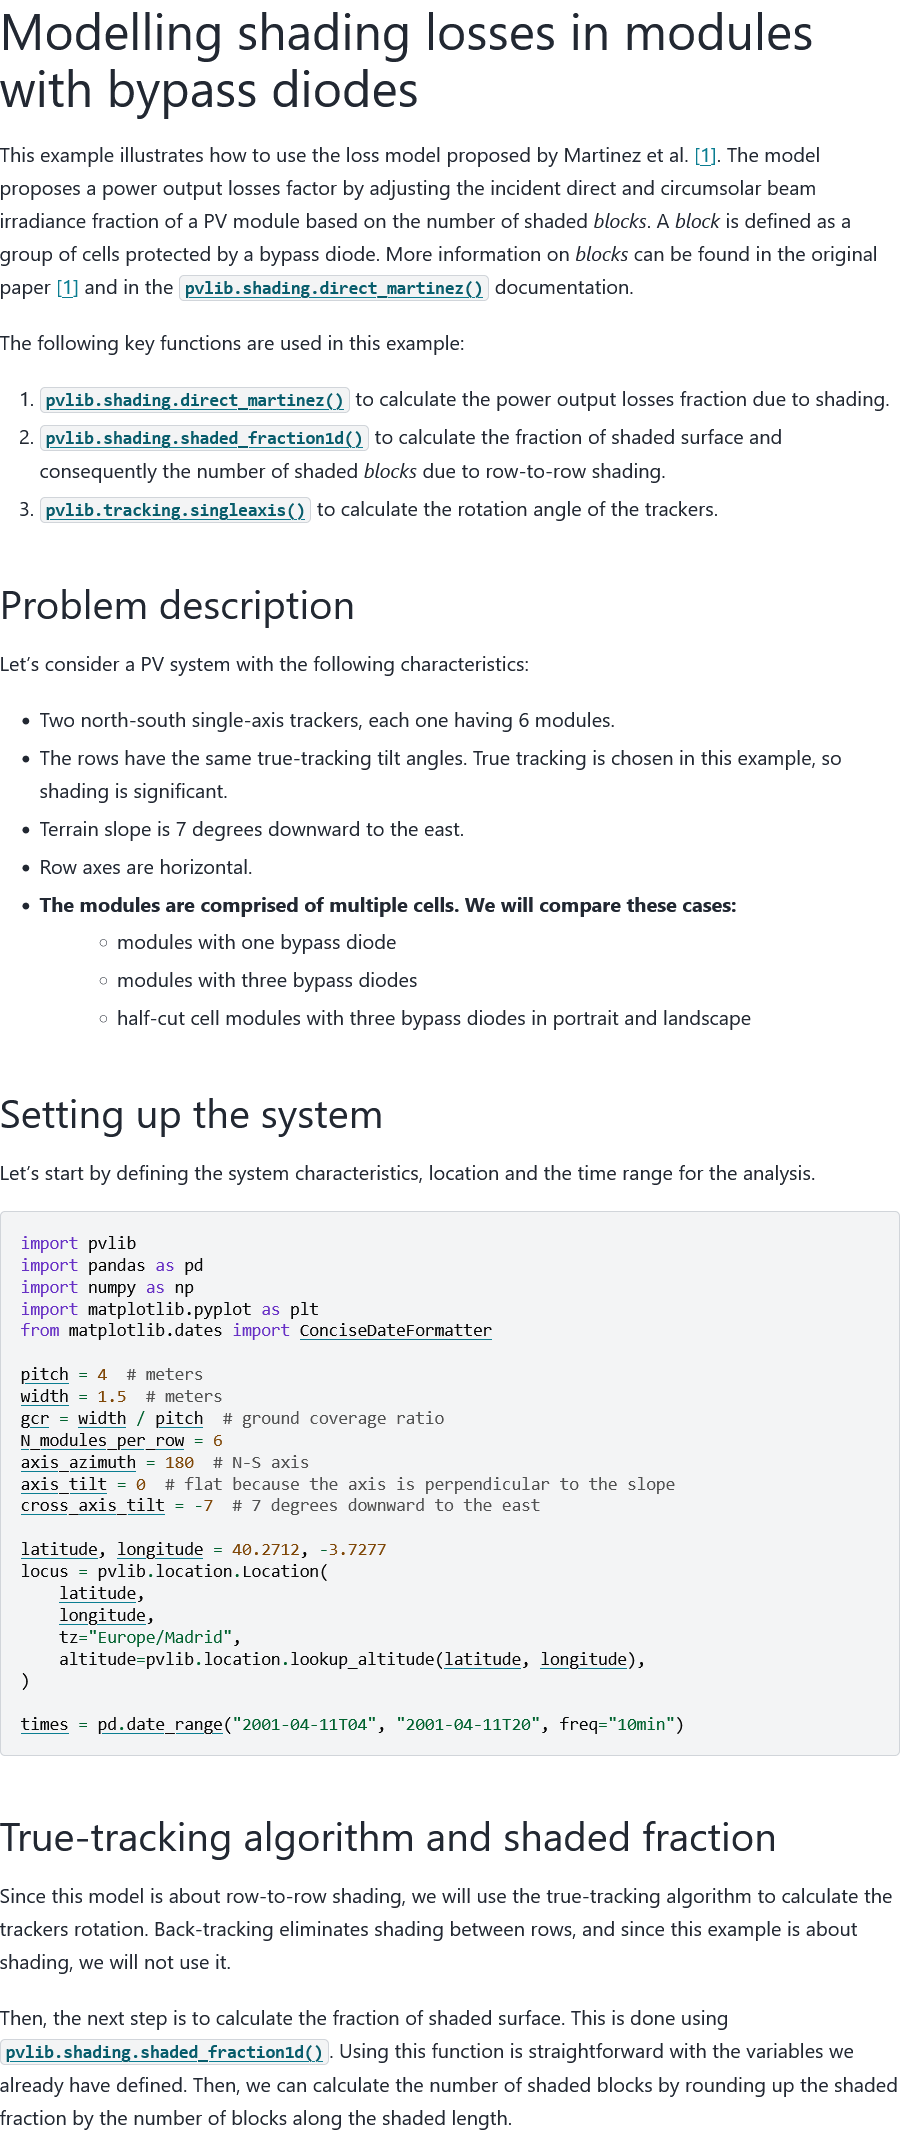
\includegraphics[width=\linewidth,height=0.9\textheight,keepaspectratio]{images/docs_examples_cut/bypass_diodes_0.png}

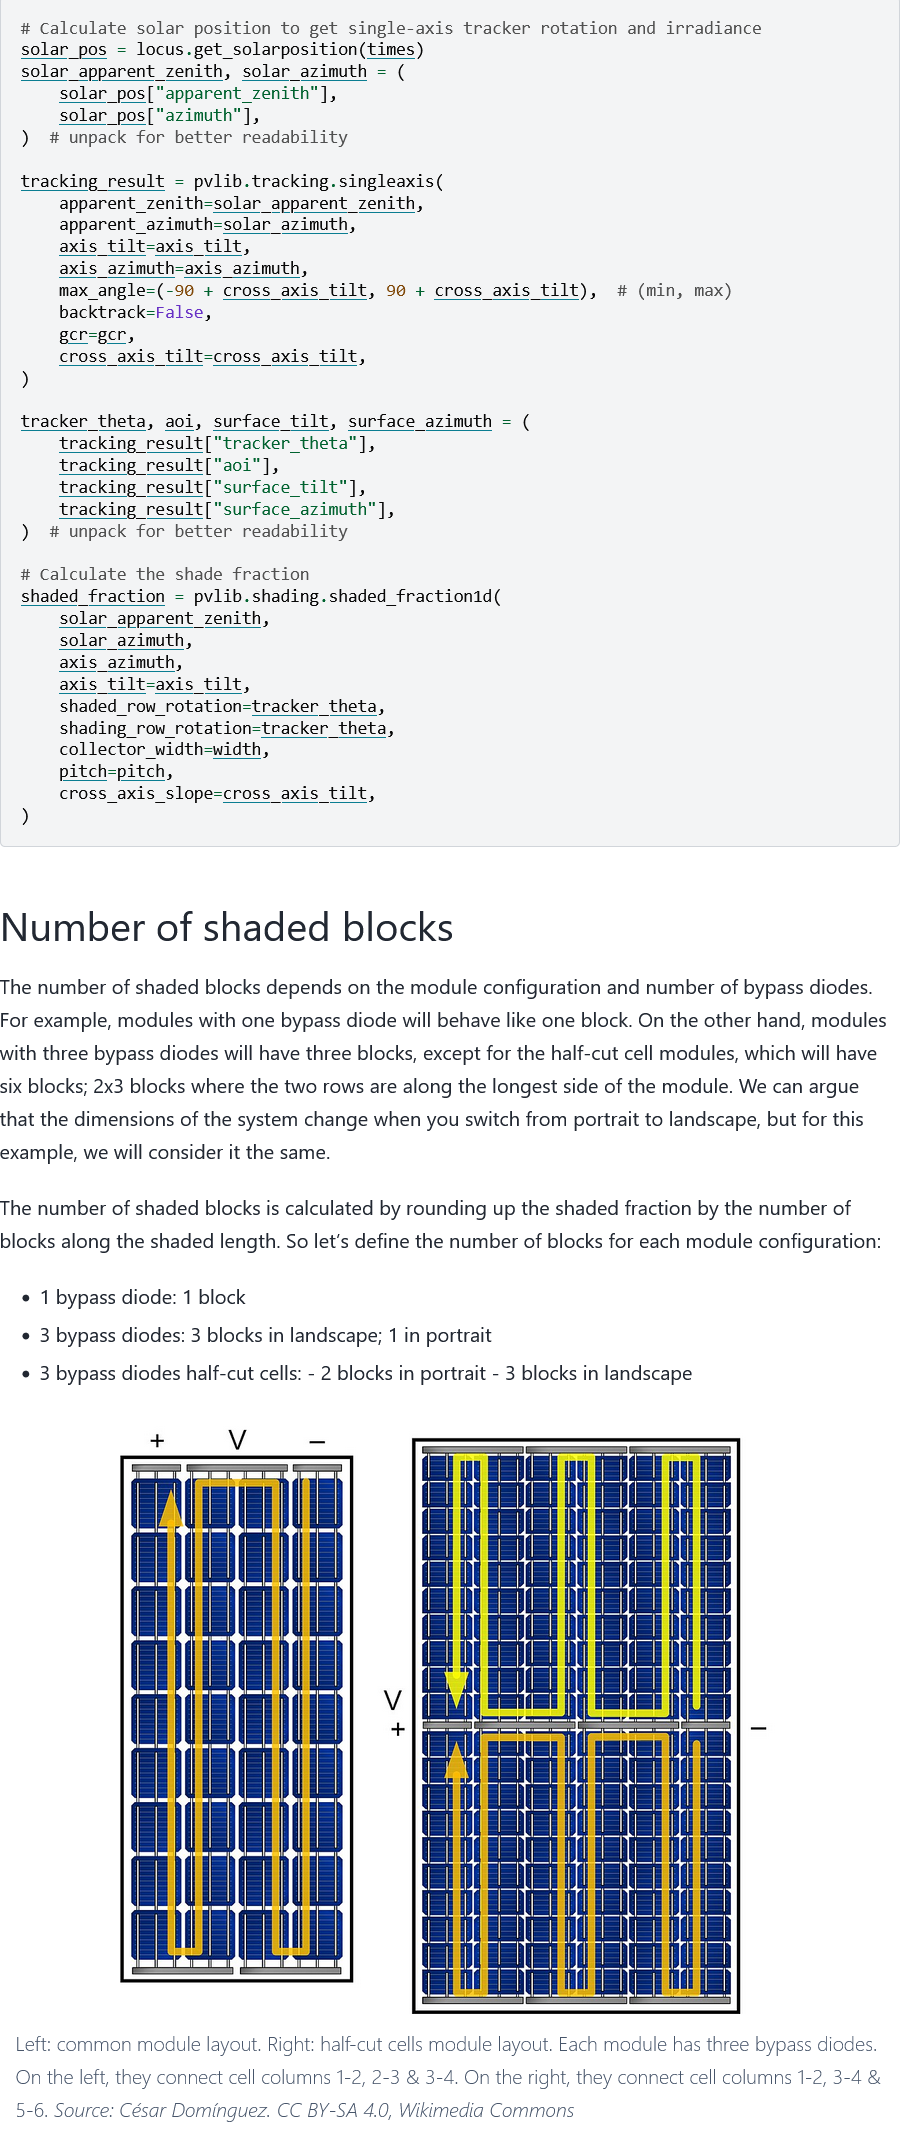
\includegraphics[width=\linewidth,height=0.9\textheight,keepaspectratio]{images/docs_examples_cut/bypass_diodes_1.png}

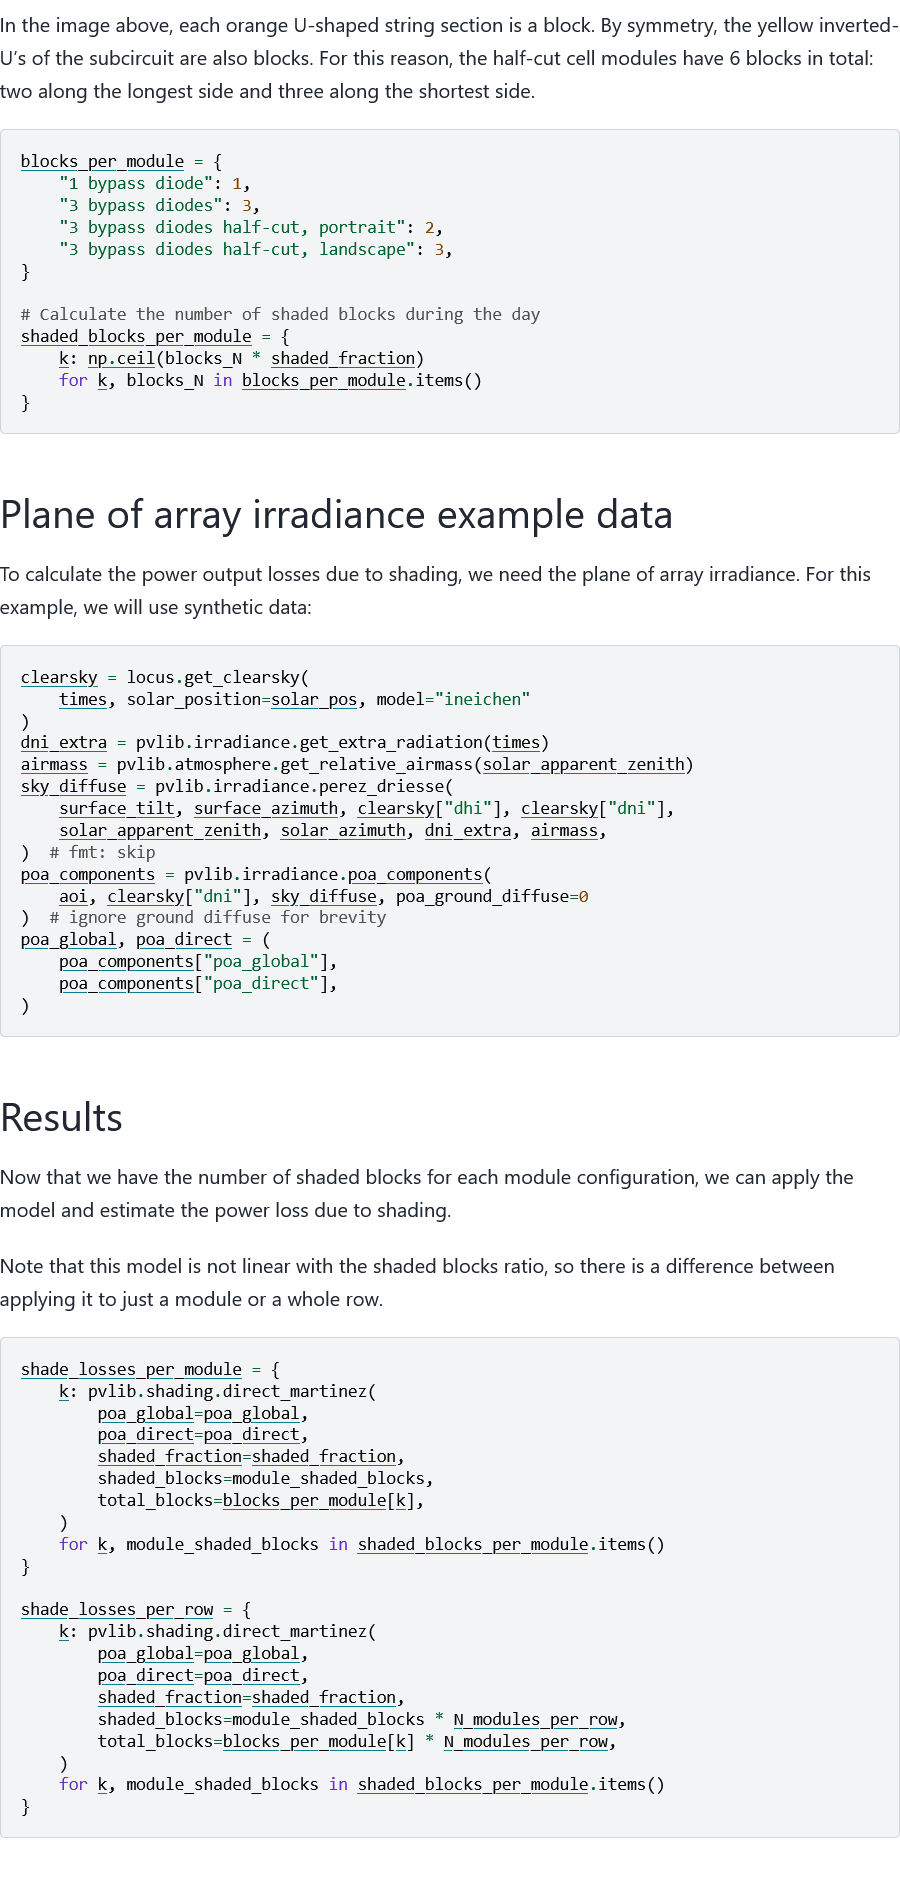
\includegraphics[width=\linewidth,height=0.9\textheight,keepaspectratio]{images/docs_examples_cut/bypass_diodes_2.png}

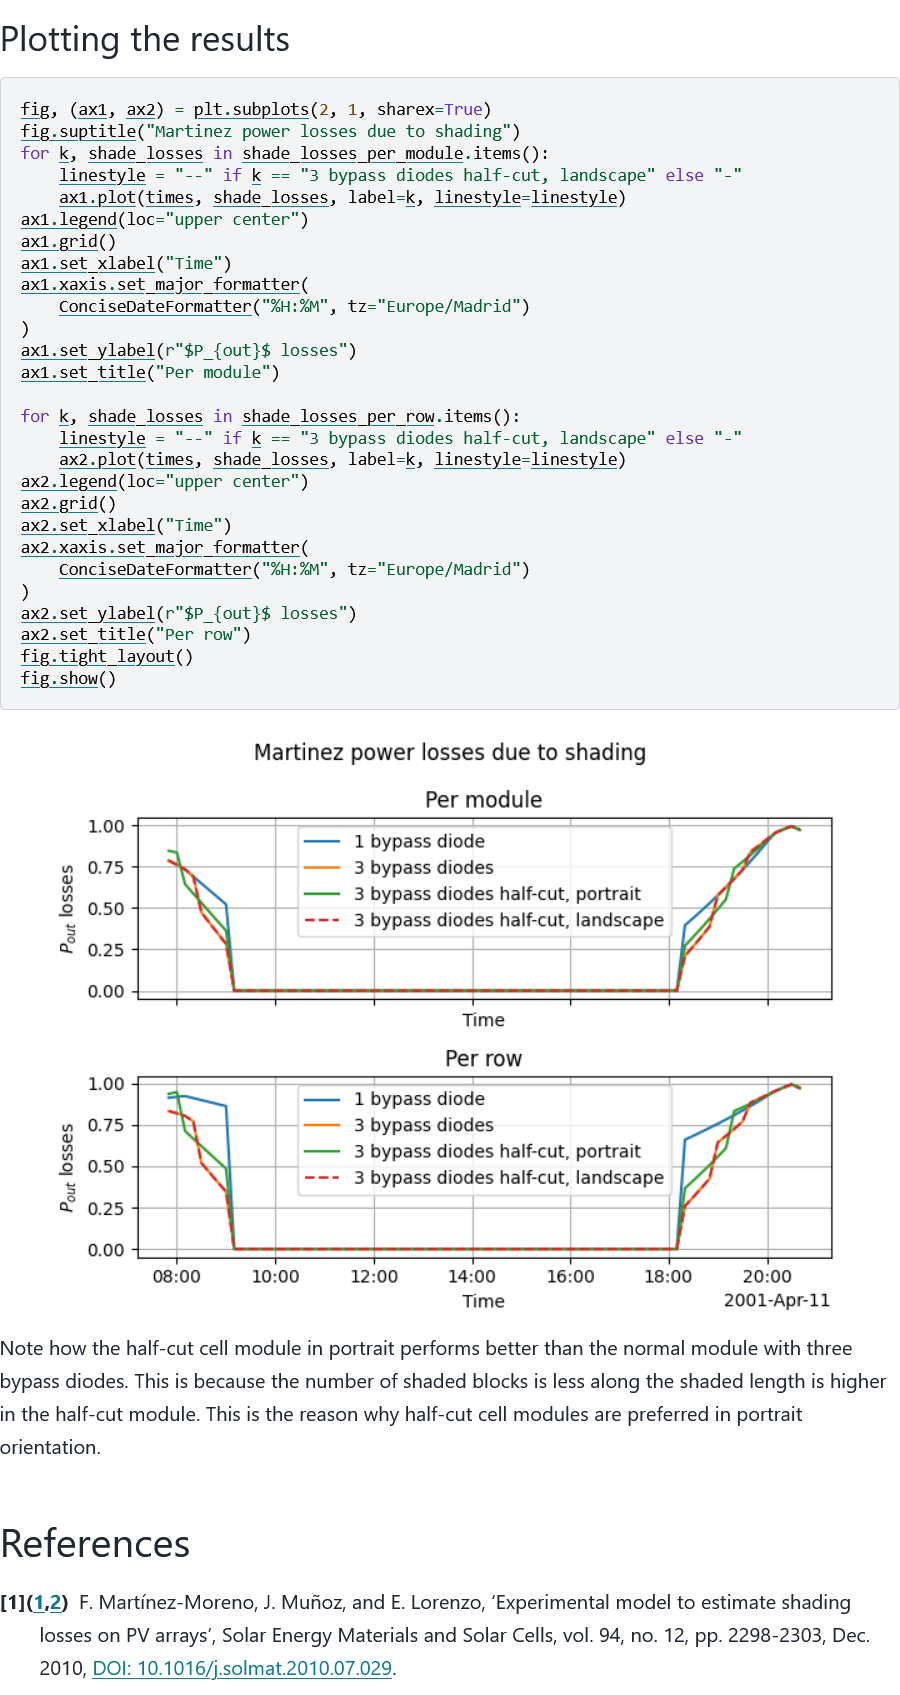
\includegraphics[width=\linewidth,height=0.9\textheight,keepaspectratio]{images/docs_examples_cut/bypass_diodes_3.png}

\newpage\section{Fracción difusa de radiación fotosintetizable diaria} \label{sct:doc_ej_par_difusa}

\pr{2048}, acceso a ejemplo en \href{https://pvlib-python.readthedocs.io/en/latest/gallery/agrivoltaics/plot_diffuse_PAR_Spitters_relationship.html}{este link}.

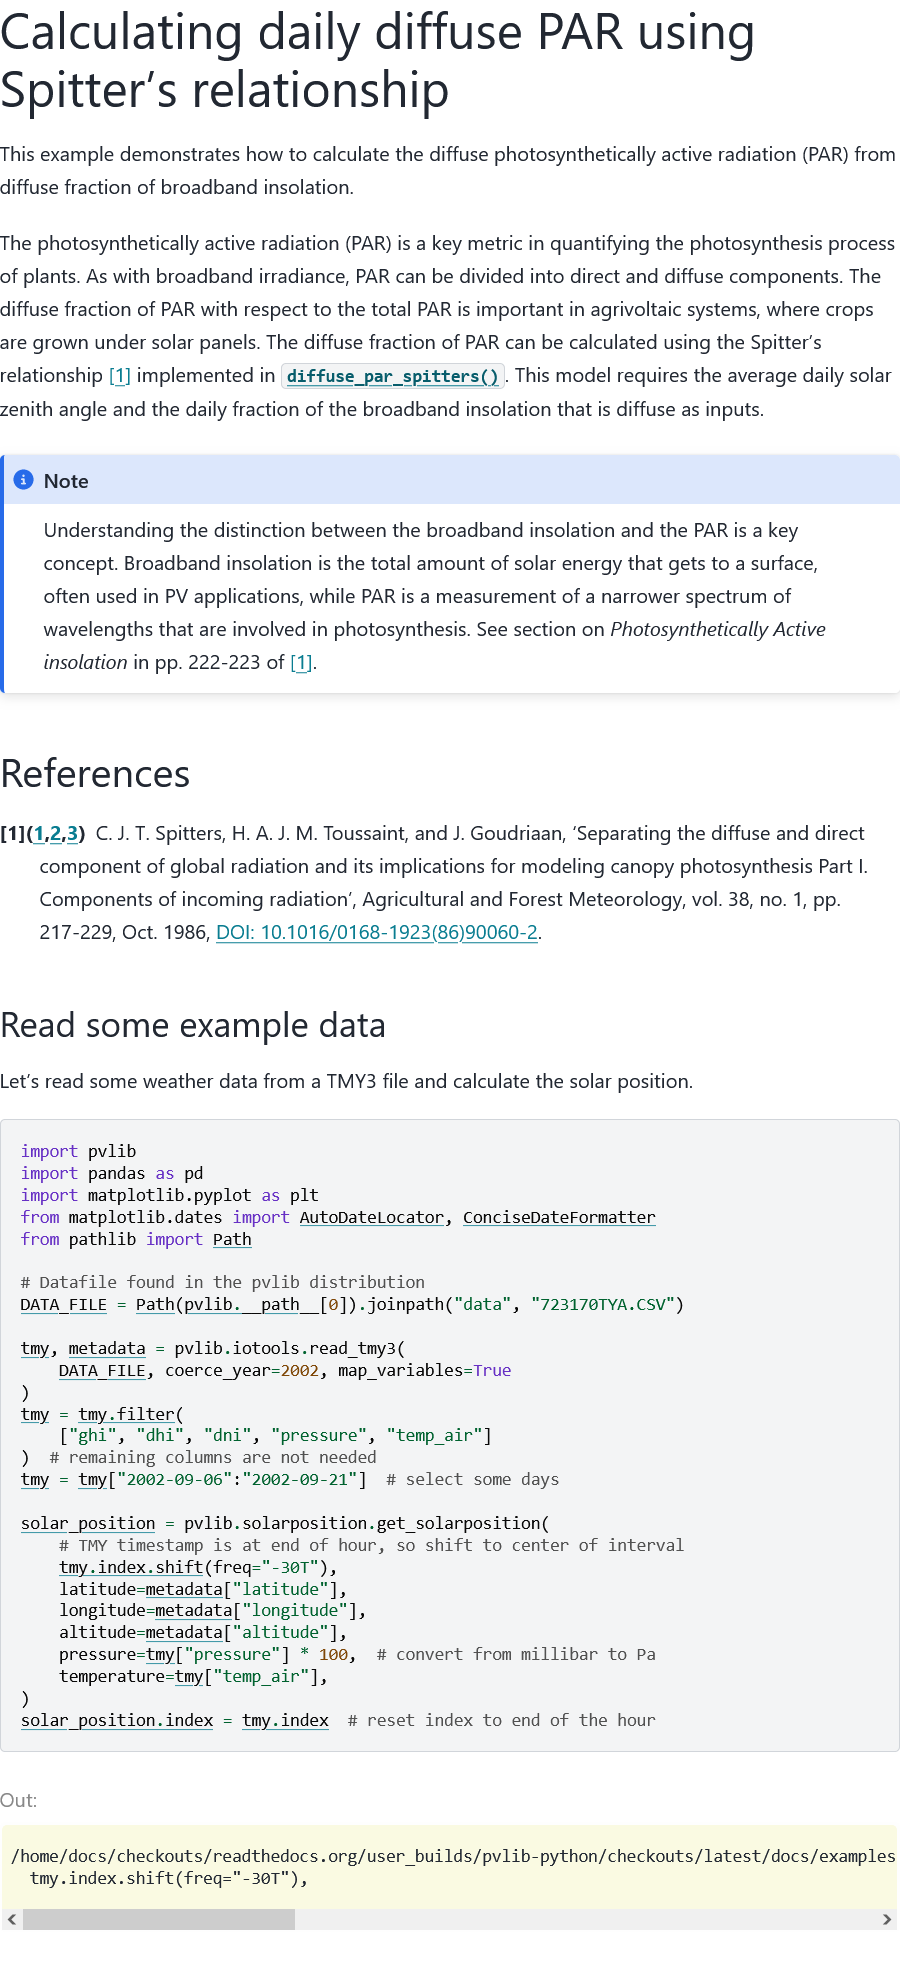
\includegraphics[width=\linewidth,height=0.9\textheight,keepaspectratio]{images/docs_examples_cut/spitters_0.png}

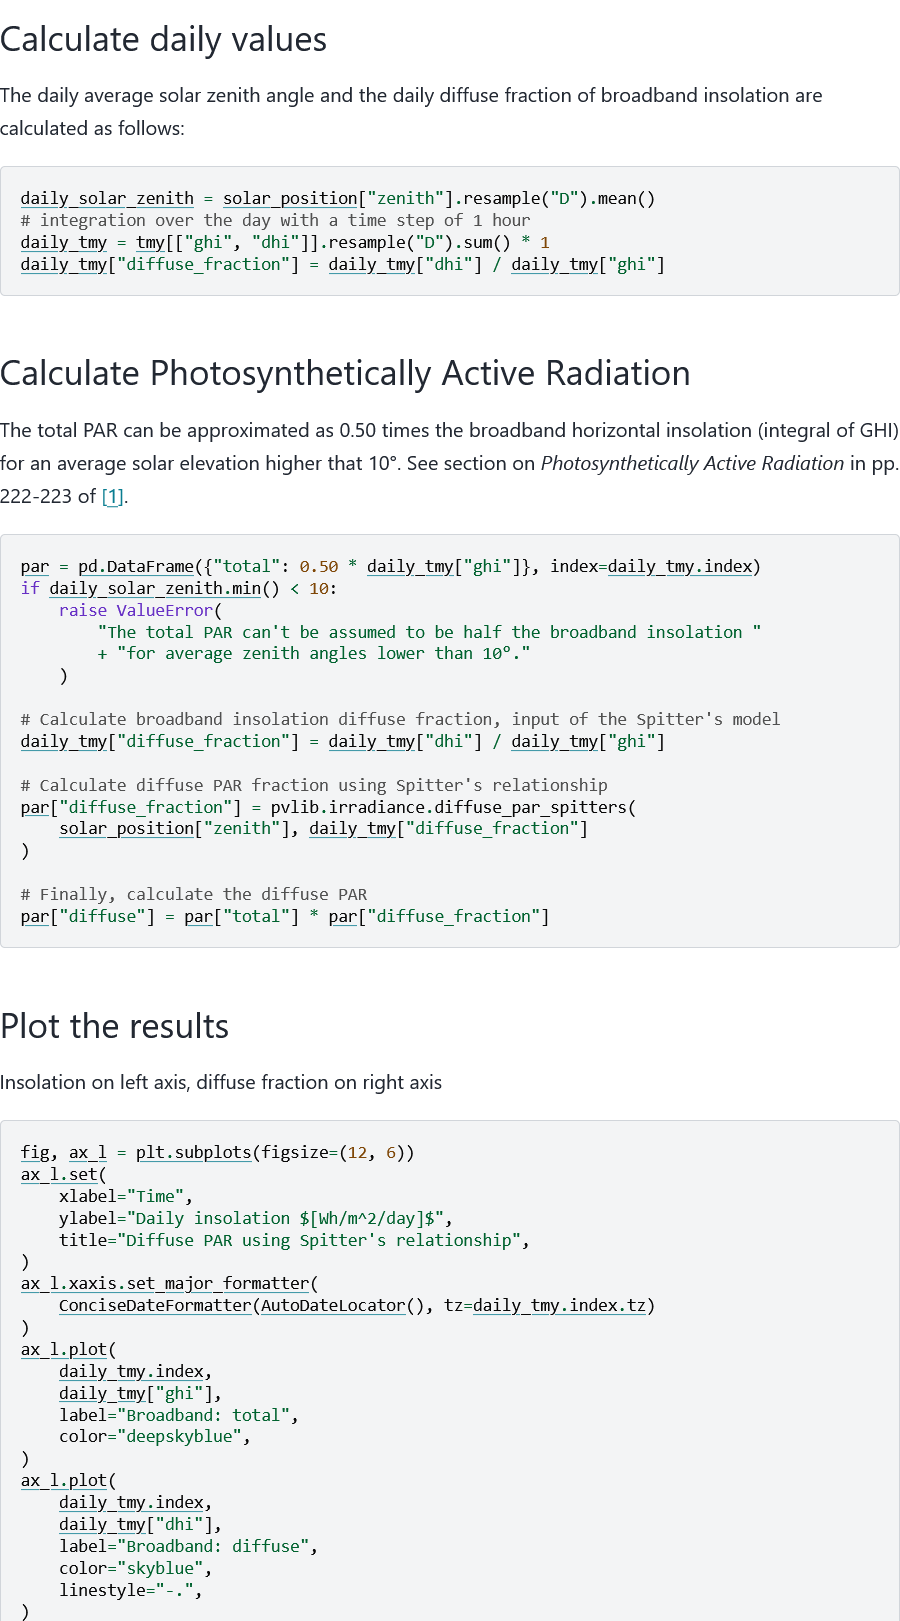
\includegraphics[width=\linewidth,height=0.9\textheight,keepaspectratio]{images/docs_examples_cut/spitters_1.png}

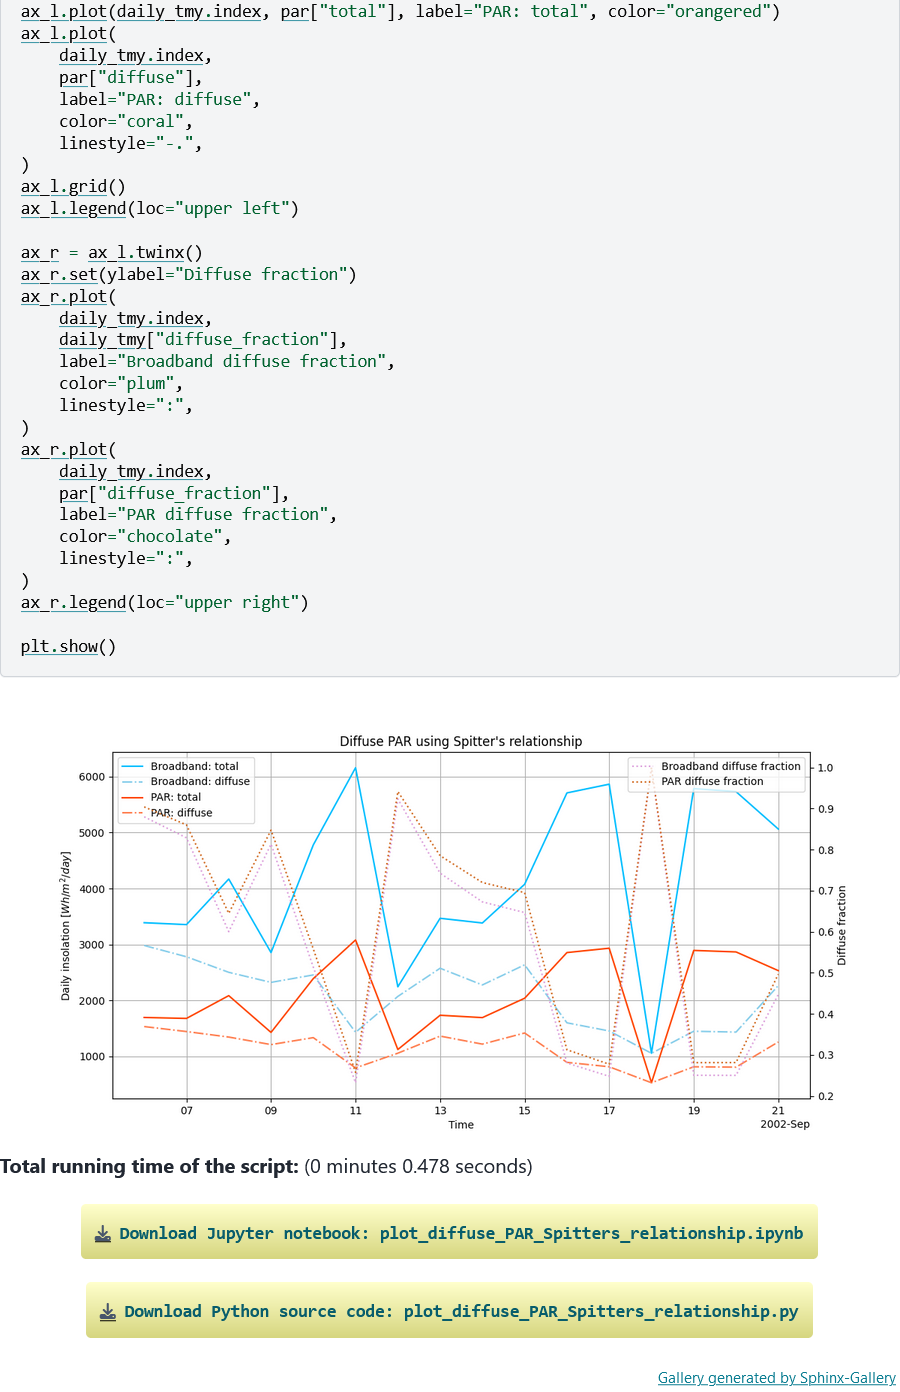
\includegraphics[width=\linewidth,height=0.9\textheight,keepaspectratio]{images/docs_examples_cut/spitters_2.png}

\newpage\section{Modelo de pérdidas por irradiancia no uniforme} \label{sct:doc_ej_modelo_ajuste_no_uniformidad}

\pr{2046}, acceso a ejemplo en \href{https://pvlib-python.readthedocs.io/en/latest/gallery/bifacial/plot_irradiance_nonuniformity_loss.html}{este link}.

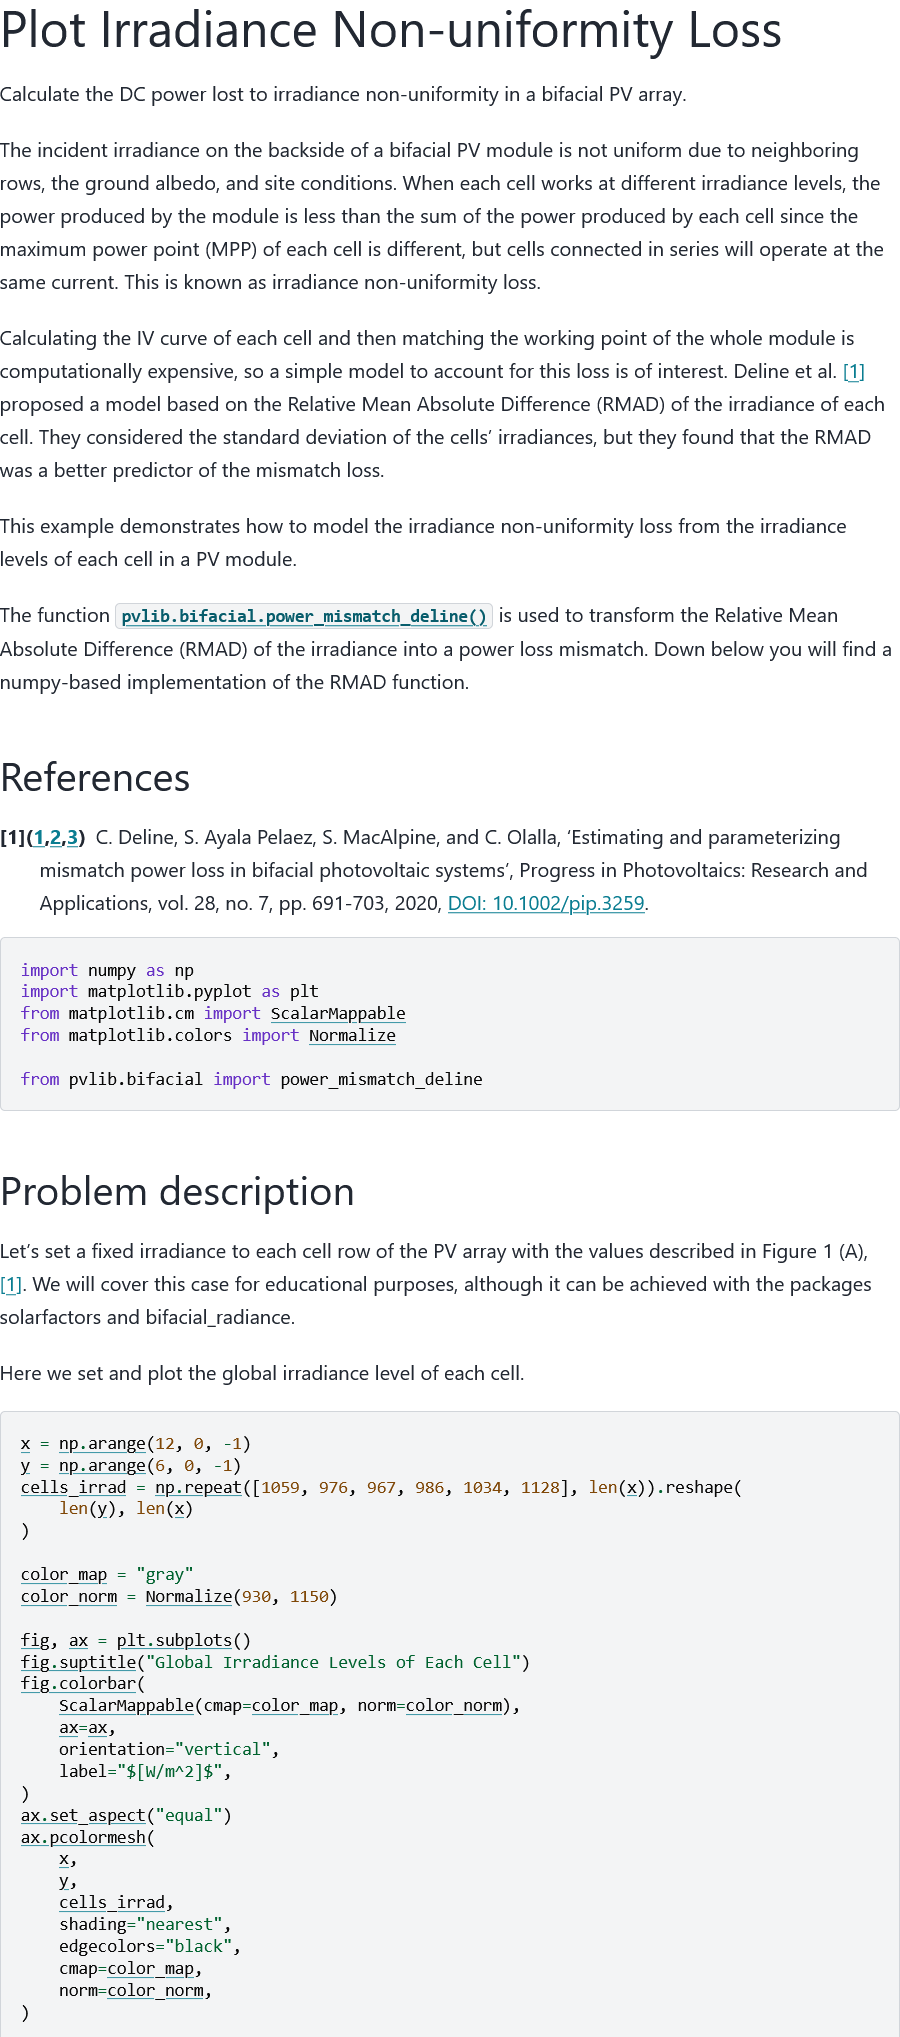
\includegraphics[width=\linewidth,height=0.9\textheight,keepaspectratio]{images/docs_examples_cut/nonuniformity_0.png}

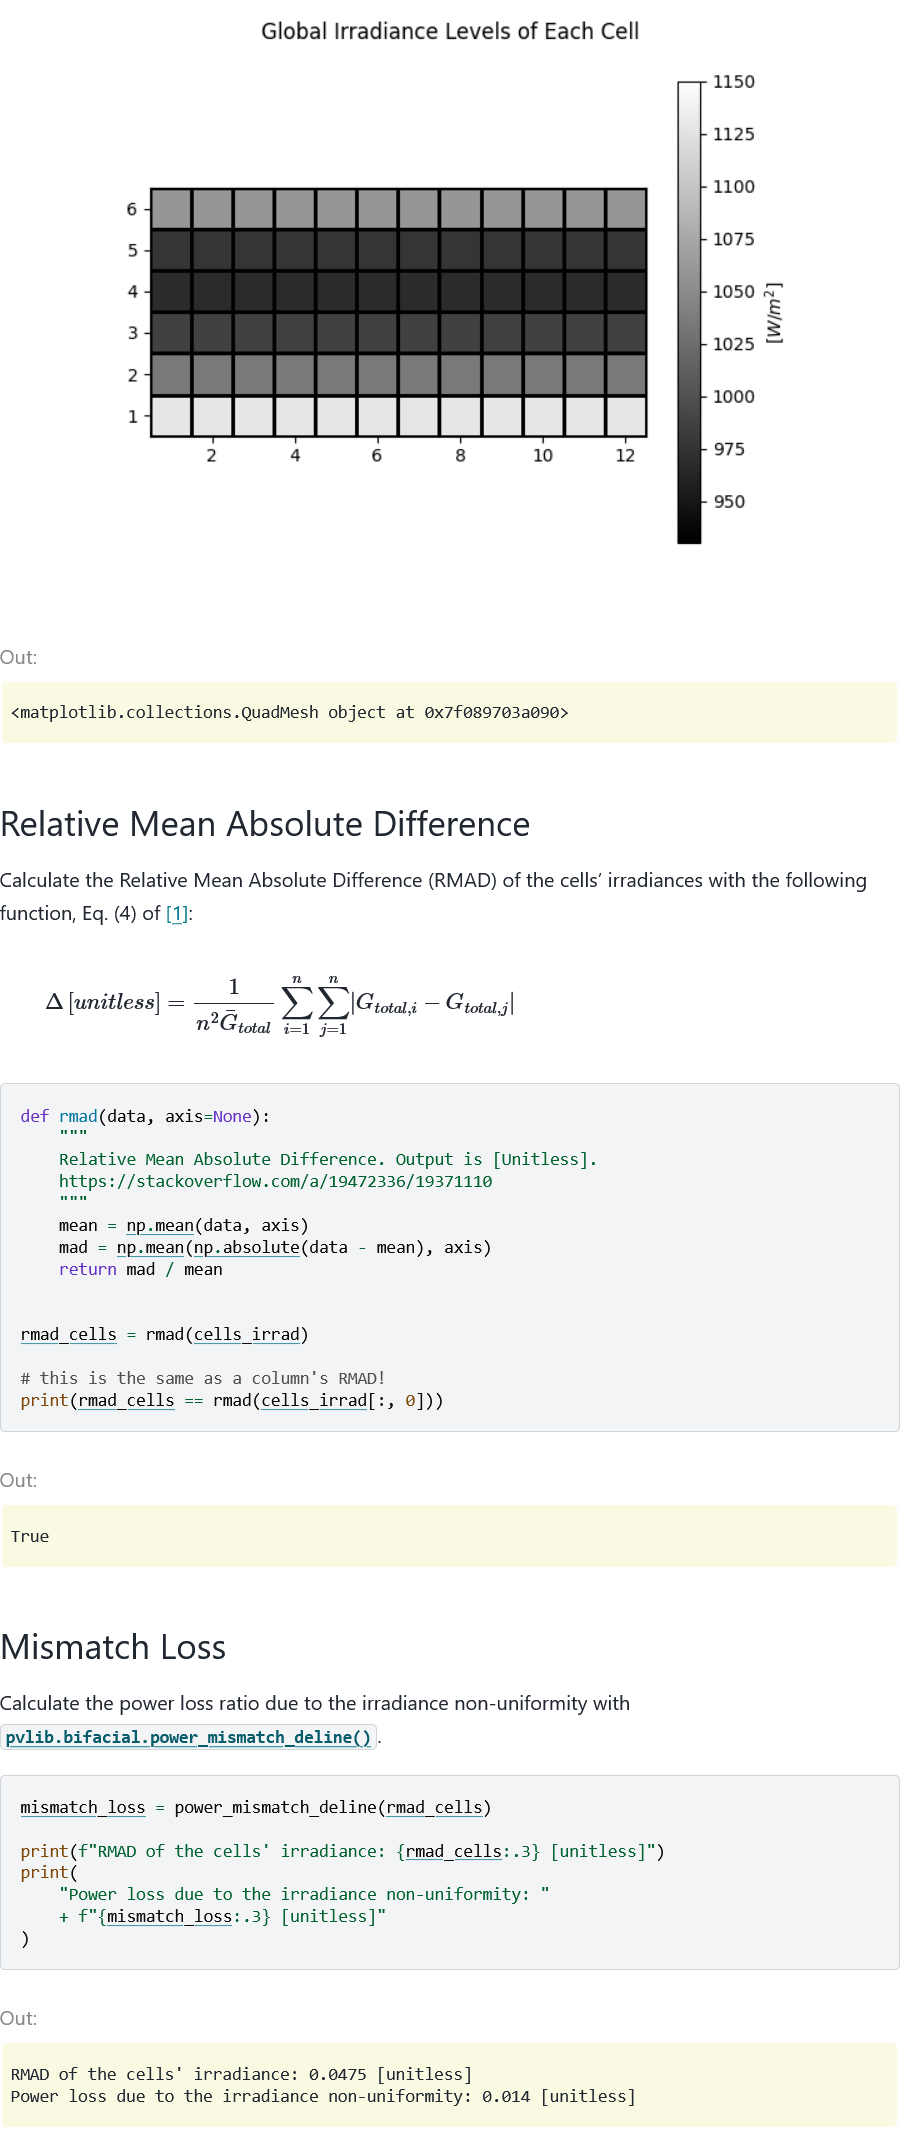
\includegraphics[width=\linewidth,height=0.9\textheight,keepaspectratio]{images/docs_examples_cut/nonuniformity_1.png}

\newpage\section{Espectro estándar ASTM G173-03} \label{sct:doc_ej_espectro_astm}

\pr{1963}, acceso a ejemplo en \href{https://pvlib-python.readthedocs.io/en/latest/gallery/spectrum/plot_standard_ASTM_G173-03.html}{este link}.

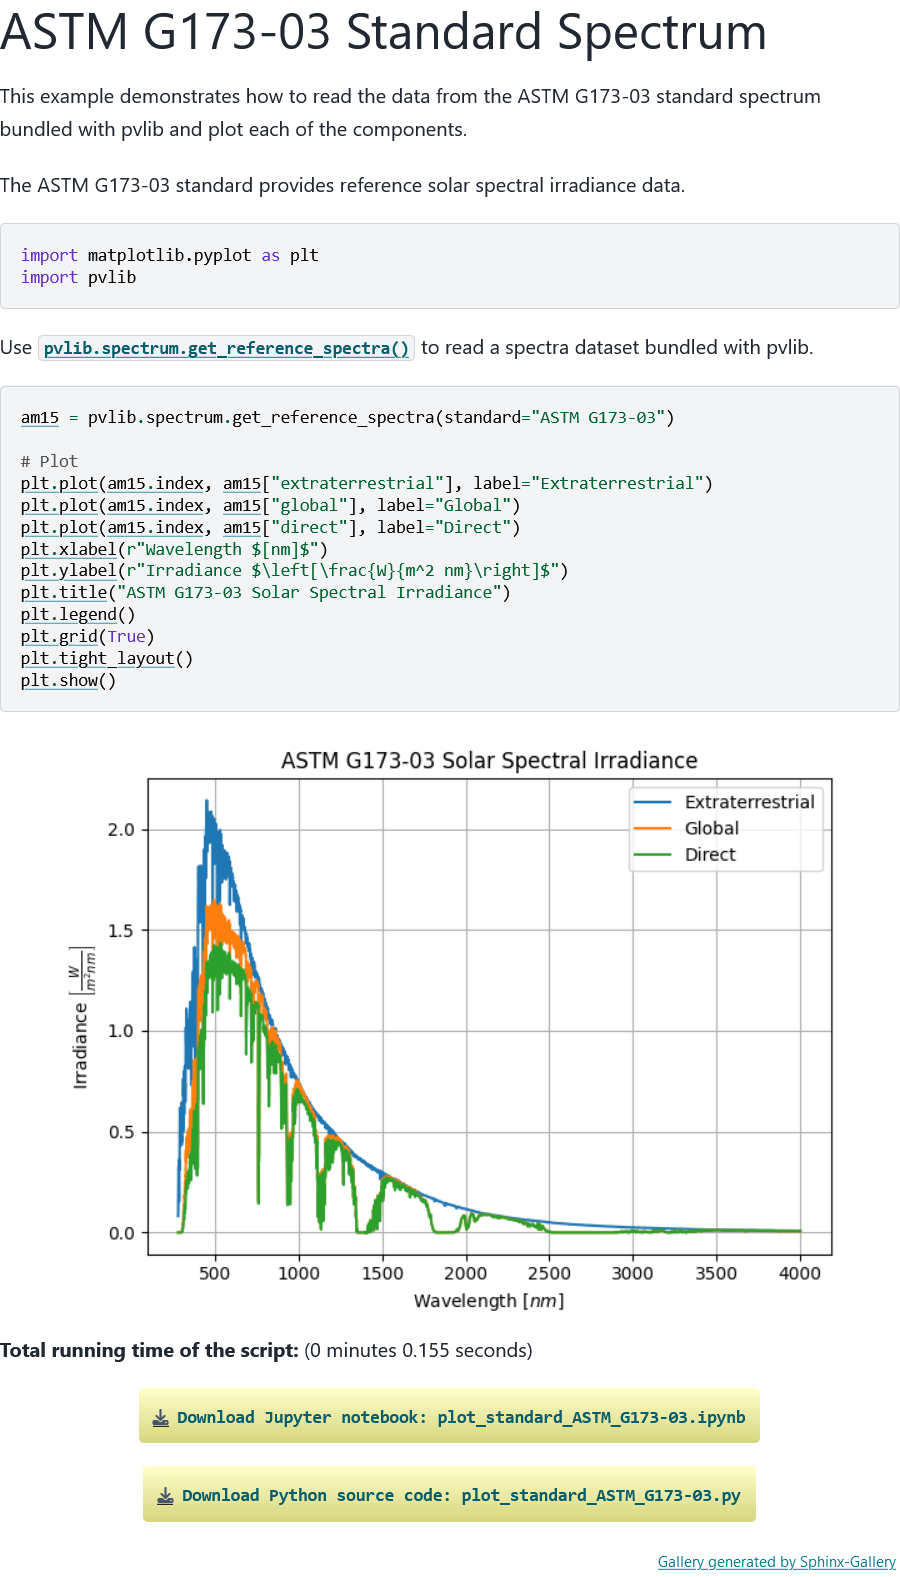
\includegraphics[width=\linewidth,height=0.9\textheight,keepaspectratio]{images/docs_examples/plot_standard_ASTM_G173-03.png}

\newpage\section{Cálculo geométrico de sombras en 3D} \label{sct:doc_ej_sombras_3d}

Propuesta en \pr{2106}, no aceptada, pero disponible temporalmente en \href{https://pvlib-python--2106.org.readthedocs.build/en/2106/gallery/shading/plot_spatial_row_to_row_shading.html}{un ejemplo de sombra estático} y \href{https://pvlib-python--2106.org.readthedocs.build/en/2106/gallery/agrivoltaics/plot_par_direct_shading0_fixed_tilt.html}{una animación de la sombra sobre un campo de cultivo}.

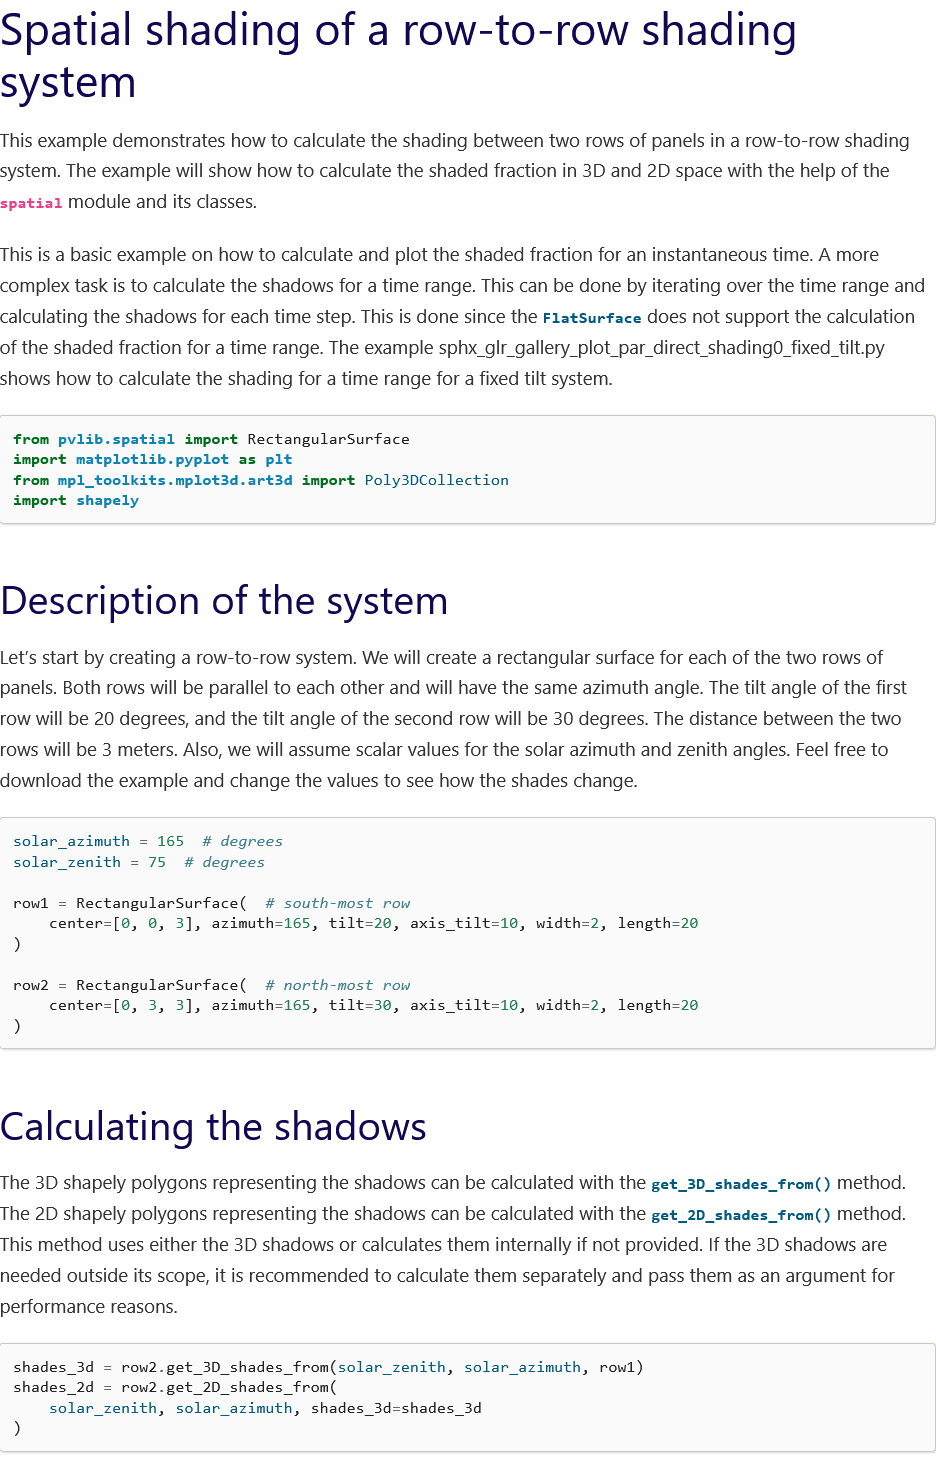
\includegraphics[width=\linewidth,height=0.9\textheight,keepaspectratio]{images/docs_examples_cut/shading_row2row_0.png}

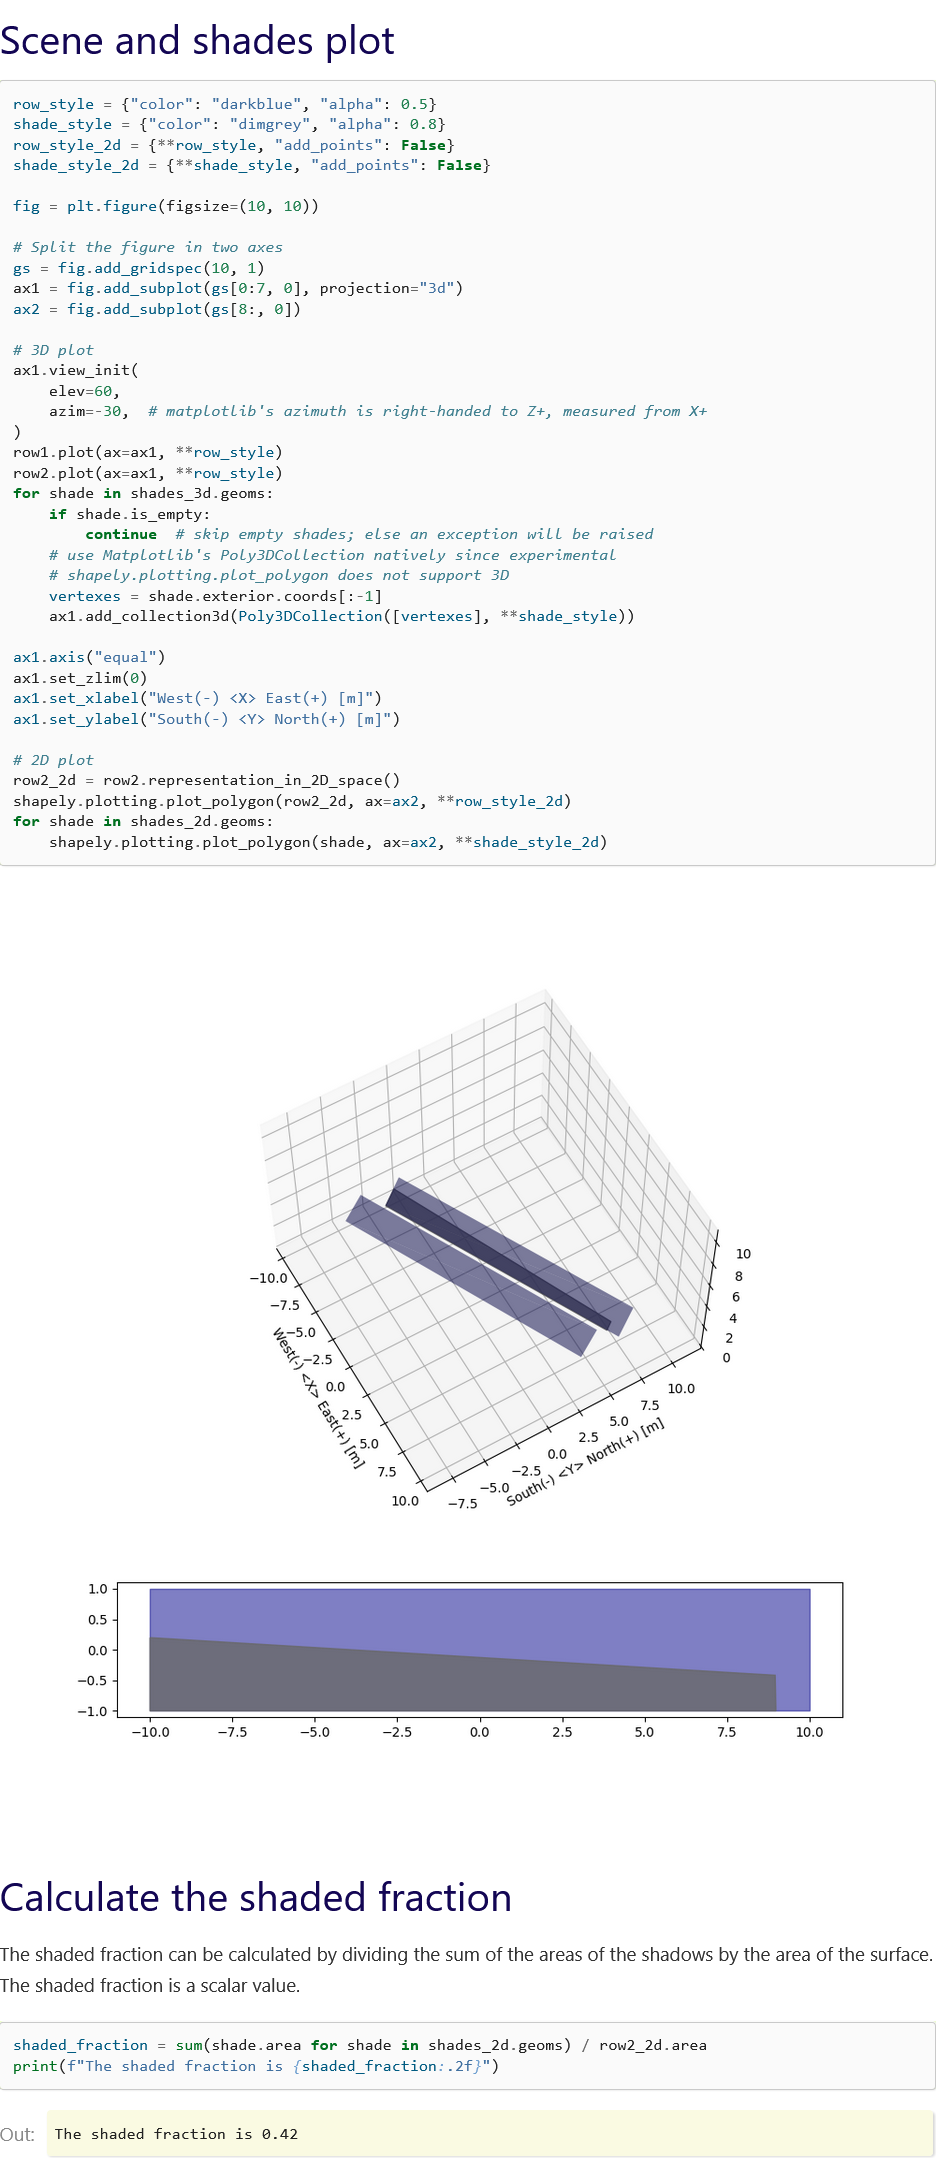
\includegraphics[width=\linewidth,height=0.9\textheight,keepaspectratio]{images/docs_examples_cut/shading_row2row_1.png}

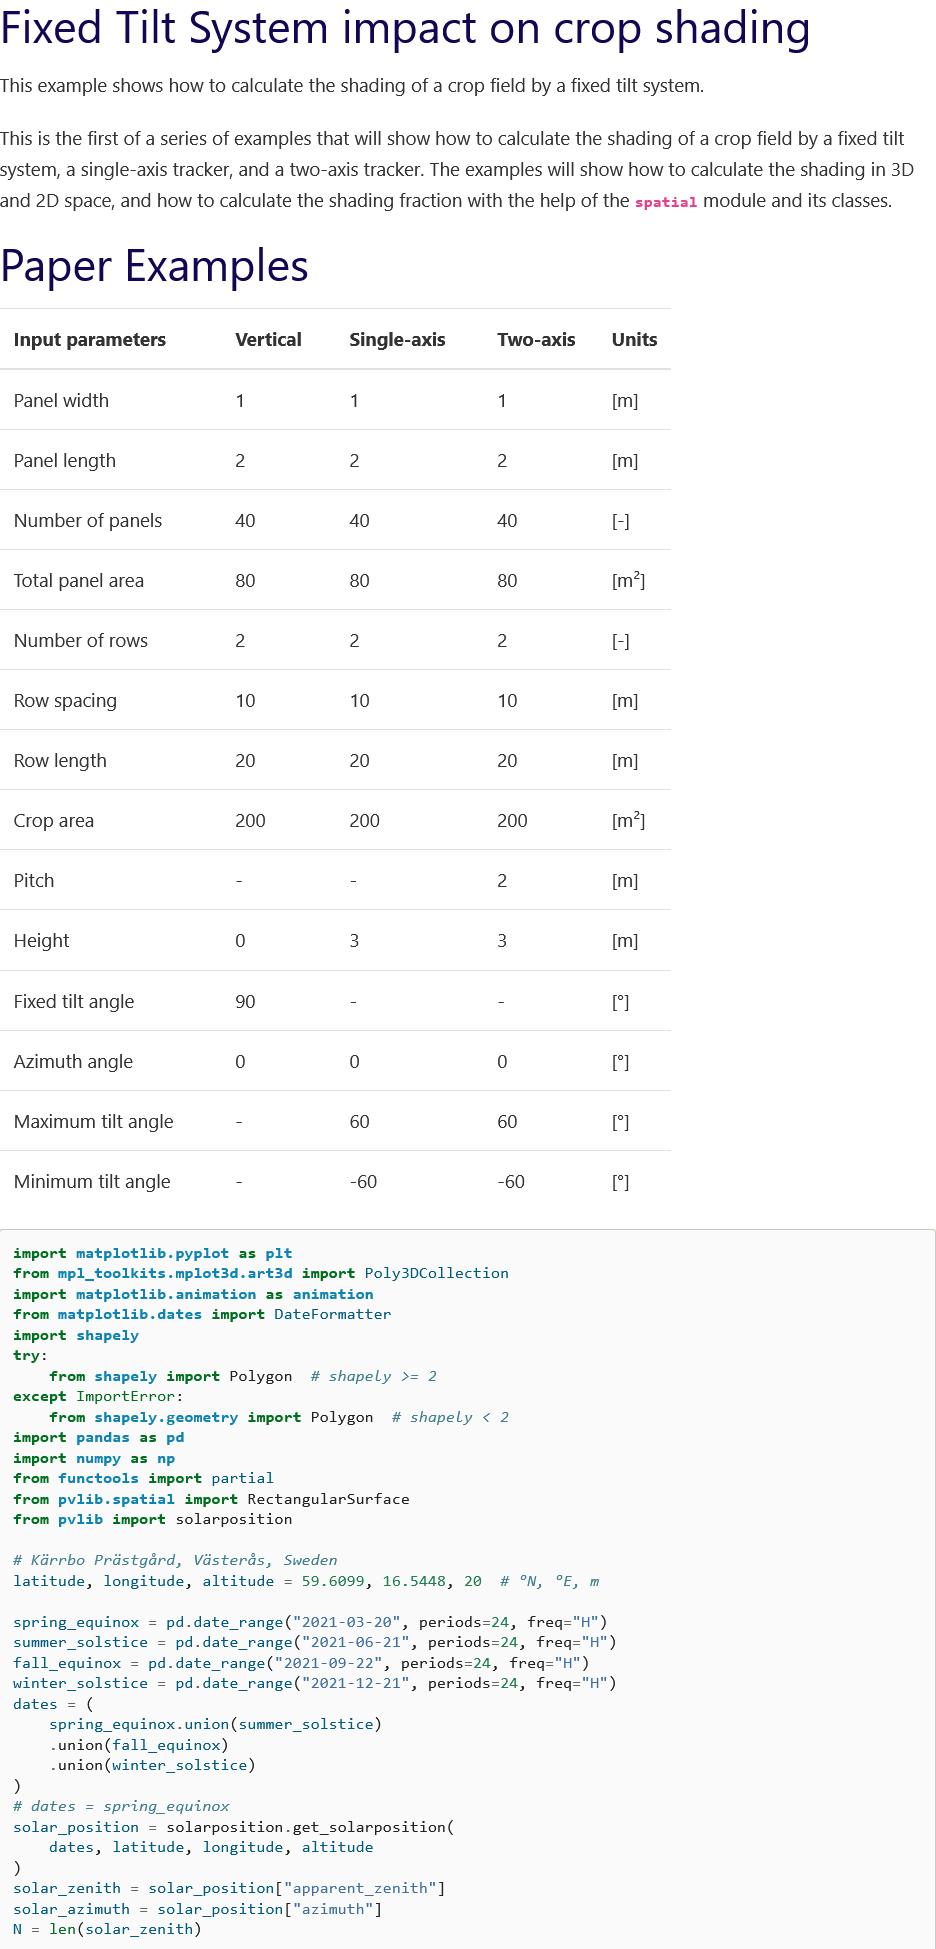
\includegraphics[width=\linewidth,height=0.9\textheight,keepaspectratio]{images/docs_examples_cut/shading_anim_0.png}

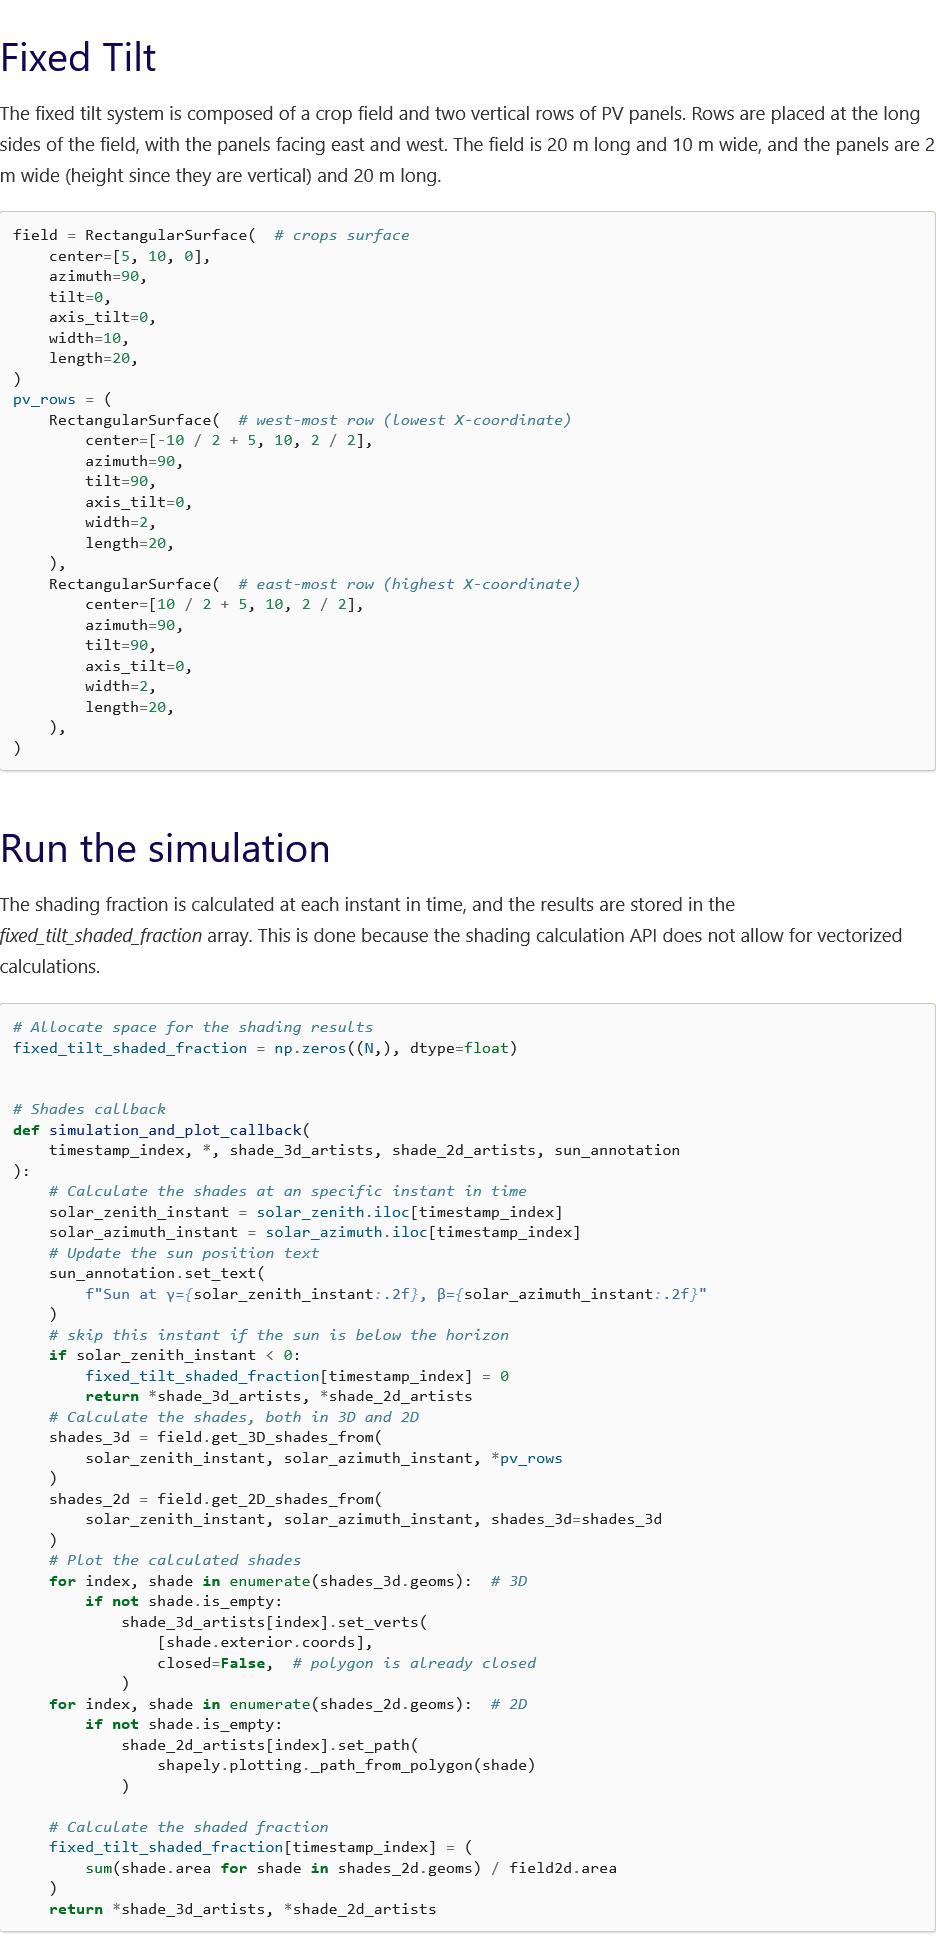
\includegraphics[width=\linewidth,height=0.9\textheight,keepaspectratio]{images/docs_examples_cut/shading_anim_1.png}

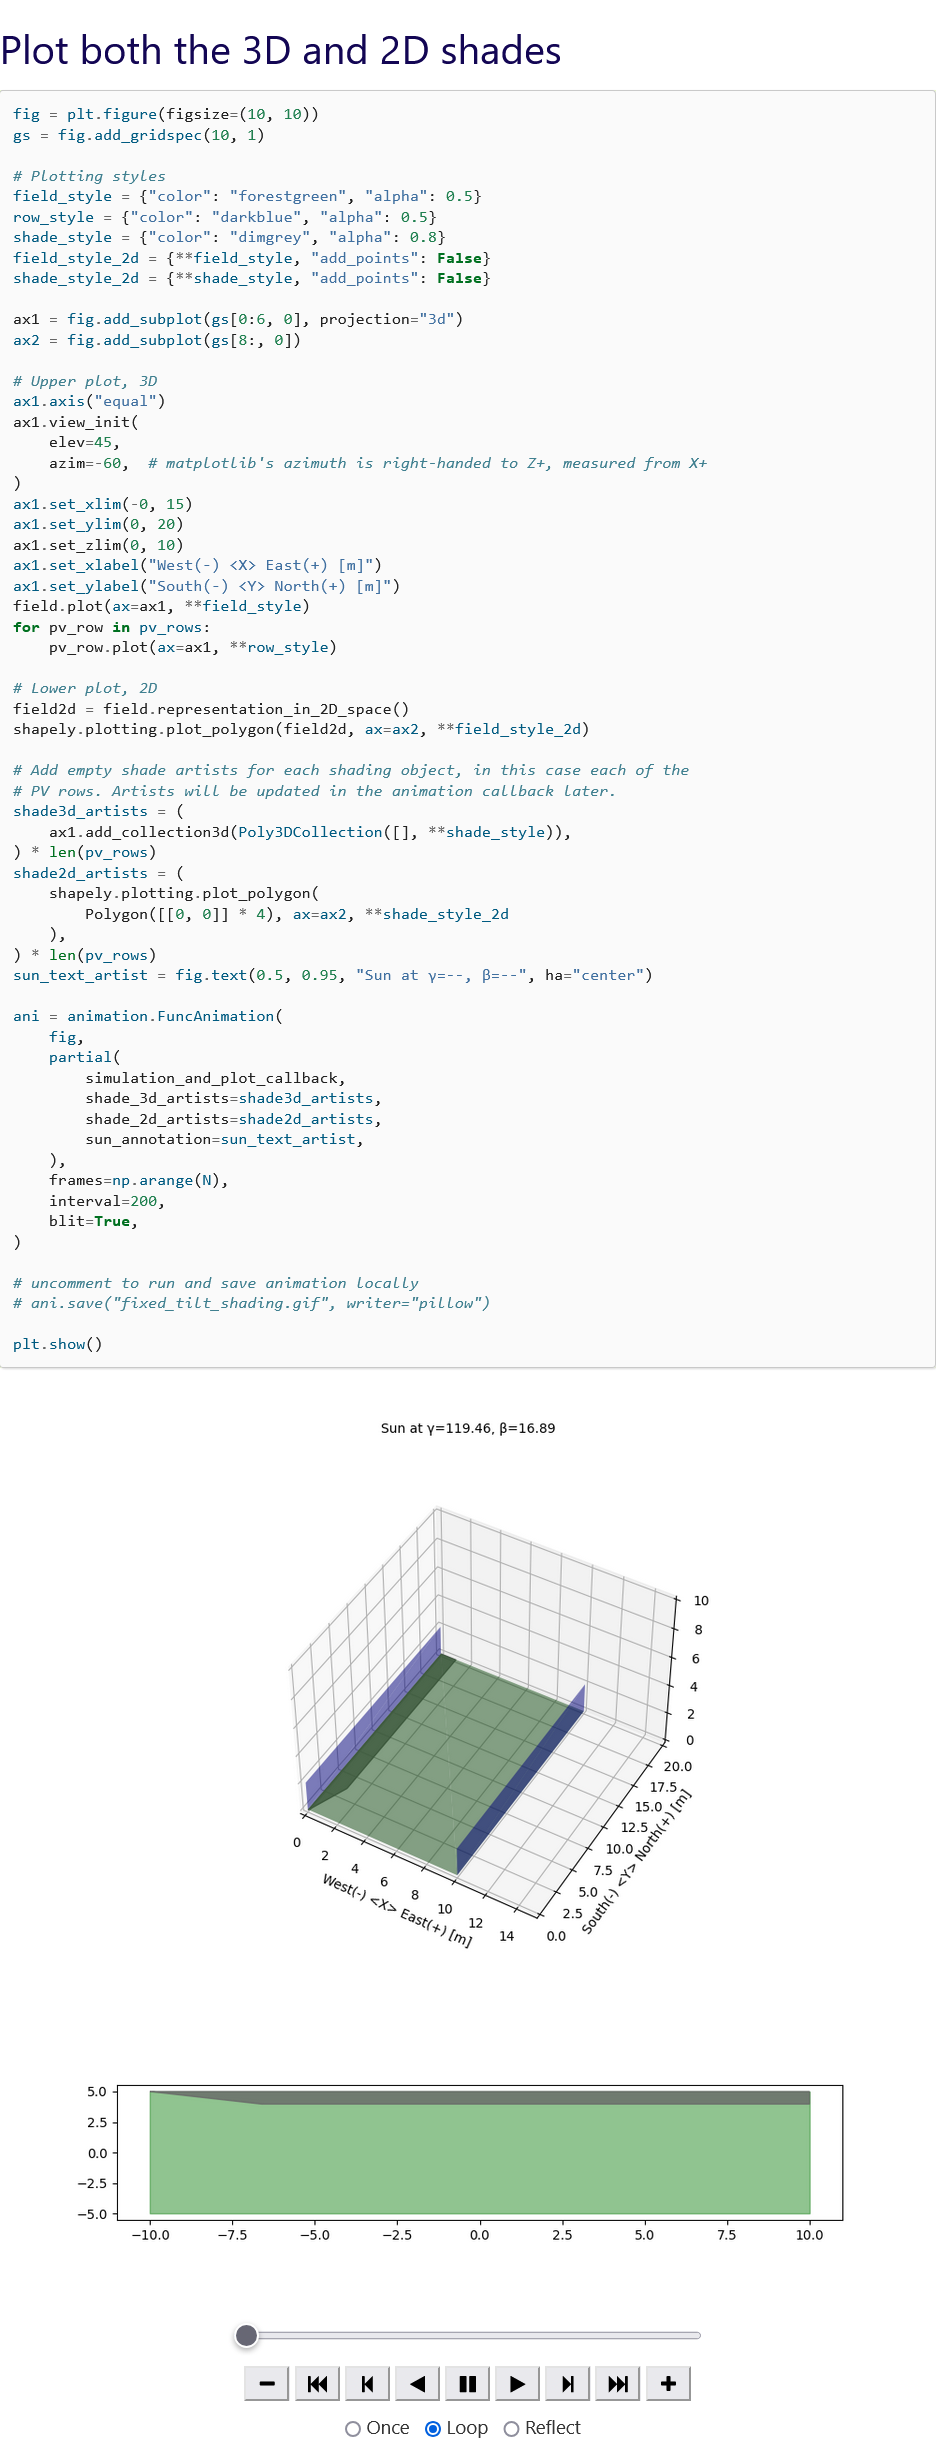
\includegraphics[width=\linewidth,height=0.9\textheight,keepaspectratio]{images/docs_examples_cut/shading_anim_2.png}

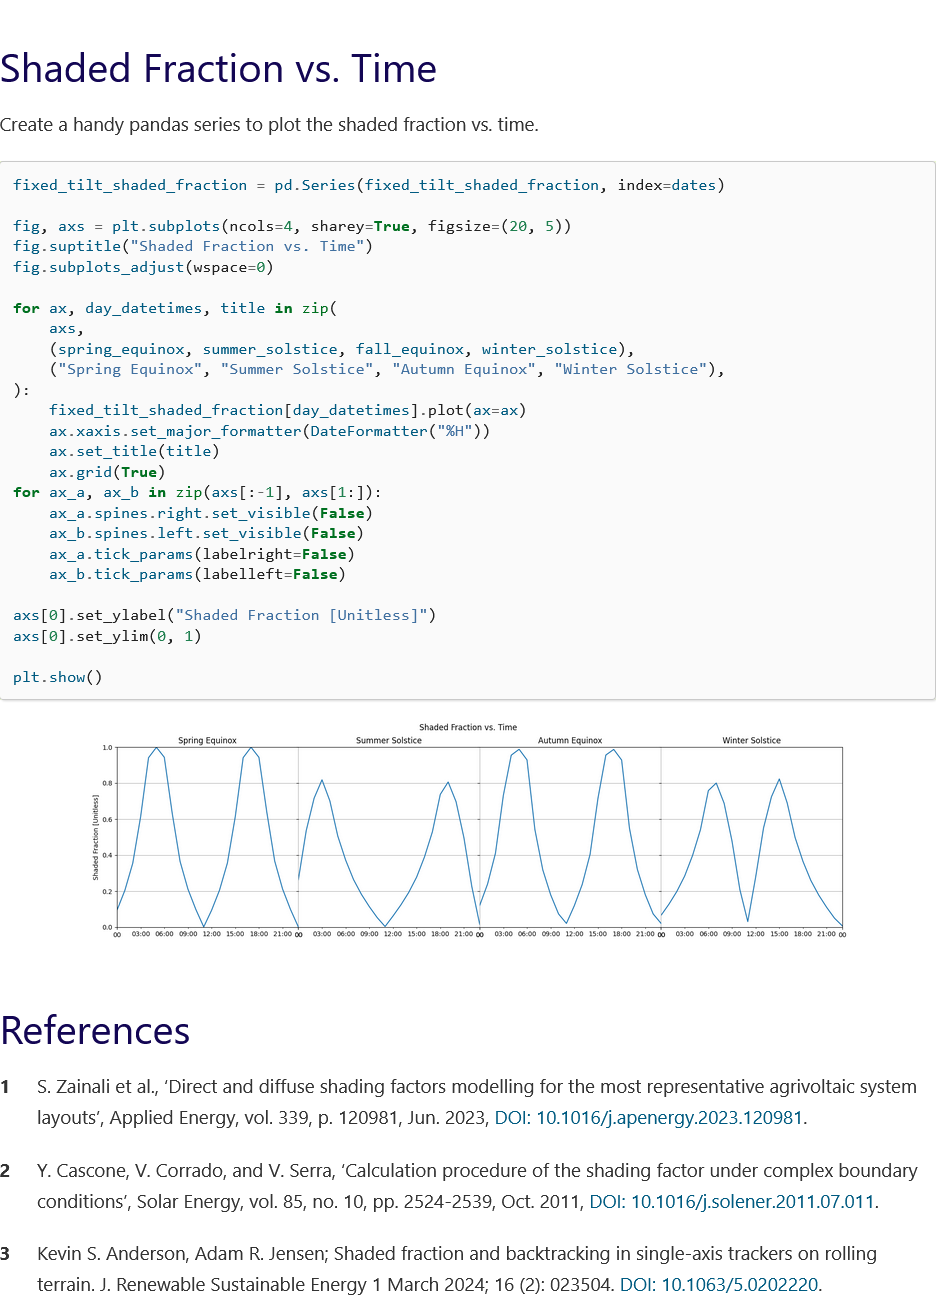
\includegraphics[width=\linewidth,height=0.9\textheight,keepaspectratio]{images/docs_examples_cut/shading_anim_3.png}

\end{myparindent}
